\documentclass[a4paper,12pt]{report}  
\usepackage{setspace}
\usepackage[french]{babel} 
\usepackage{ragged2e}
\usepackage{xcolor,graphicx}
\usepackage[top=0.6in,bottom=0.6in,right=1in,left=1in]{geometry}
\usepackage[top=0.6in,bottom=0.6in,right=1in,left=1in]{geometry}
\usepackage[T1]{fontenc}
\usepackage[utf8]{inputenc}
\usepackage[utf8]{inputenc}
\usepackage{xcolor,graphicx}
\usepackage{fancyhdr}
\usepackage{listings}
\usepackage{array}
\usepackage{adjustbox}
\usepackage[colorlinks, allcolors=black]{hyperref}
\usepackage{lipsum}
\usepackage{amsmath}
\usepackage{caption}
\usepackage{enumitem}

\setlength{\headheight}{14.61858pt}
\definecolor{blue}{RGB}{31,56,100}
\hypersetup{
    pdftitle={Titre de la mémoire},    % Titre 
    pdfauthor={Nom Prénom},    % Auteur
    pdfsubject={Domaine},   % Sujet 
    pdfkeywords={keyword1, keyword2},   % liste Mot clés
}

%%%%%%%%%%%%%%%%%%%%%%%%%%%%%%%%%%%%%%%%%%%%%%%%%%%%%%%%%%%%%%%%%%%%%%%%%%%%%
%%%%%%%%%%%%%%%%%%%%%%%%%%%%%%%%%%%%%%%%%%%%%%%%%%%%%%%%%%%%%%%%%%%%%%%%%%%%
%% Modifier Selon vos informations visibles (Choisir un titre bref et précis)
\newcommand{\mytitle}{Système de recommandation de cours éducatifs basé sur l'IA générative}
\newcommand{\myname}{M. Zarouala Abdellah}
\newcommand{\mylogo}{\includegraphics[height=1.8cm]{./images/Ste_logo.jpg}} 

%%%%%%%%%%%%%%%%%%%%%%%%%%%%%%%%%%%%%%%%%%%%%%%%%%%%%%%%%%%
% Numérotation des sections de début
\fancypagestyle{firstpages}{
    \fancyhf{}  
    \renewcommand{\headrulewidth}{0pt}  
      
    \pagenumbering{arabic}  
}

% Numérotation des chapitres
 

% Style pour le code listings
\definecolor{codegreen}{rgb}{0,0.6,0}
\definecolor{codegray}{rgb}{0.5,0.5,0.5}
\definecolor{codepurple}{rgb}{0.58,0,0.82}
\definecolor{backcolour}{rgb}{0.95,0.95,0.92}

\lstdefinestyle{mystyle}{
    backgroundcolor=\color{backcolour},   
    commentstyle=\color{codegreen},
    keywordstyle=\color{magenta},
    numberstyle=\tiny\color{codegray},
    stringstyle=\color{codepurple},
    basicstyle=\ttfamily\footnotesize,
    breakatwhitespace=false,         
    breaklines=true,                 
    captionpos=b,                    
    keepspaces=true,                 
    numbers=left,                    
    numbersep=5pt,                  
    showspaces=false,                
    showstringspaces=false,
    showtabs=false,                  
    tabsize=2
}
\lstset{style=mystyle}


%%%%% Profendeur des sections
\setcounter{tocdepth}{3}
\setcounter{secnumdepth}{3}

\begin{document}
%%%%%%%%%%%%%%%%%%%%%%%%%%%%%%%%%%%%%%%%%%%%%%%%%%%%%%%%%%%%%%%%%%%%%%%%%%%%%%
%%%%%%%%%%%%%%%%%%%%%%%%%%%%%%%%%%%%%%%%%%%%%%%%%%%%%%%%%%%%%%%%%%%%%%%%%%%%%%
% Page de Garde
%%%%%%%%%%%%%%%%%%%%%%%%%%%%%%%%%%%%%%%%%%%%%%%%%%%%%%%%%%%%%%%%%%%%%%%%%%%%%
%%%%%%%%%%%%%%%%%%%%%%%%%%%%%%%%%%%%%%%%%%%%%%%%%%%%%%%%%%%%%%%%%%%%%%%%%%%%%
%%%% Entéte Logo de l'université Mohammed V - Faculté des sciences Rabat
\begin{titlepage}
    \begin{center}
        \begin{minipage}{3cm}
            \begin{center}
            \includegraphics[height=1.8cm]{./images/Logo_FSR.jpg}
            \end{center}
        \end{minipage} \hfill
        \begin{minipage}{9cm}
            \begin{center}
            \textbf{UNIVERSITÉ MOHAMMED V }\\[0.1cm]
            \textbf{FACULTÉ DES SCIENCES RABAT}\\[0.1cm]
            \textbf{DÉPARTEMENT D'INFORMATIQUE}
            \end{center}
        \end{minipage}\hfill
        \begin{minipage}{3cm}
            \begin{center}
            \includegraphics[height=1.3cm]{./images/Logo_MSID_invisible.png}
        \end{center}
        \end{minipage}
    %%%%%%%%%%%%%%%%%%%%%%%%%%%%%%%%%%%%%%%%%%%%%%%%%%%%%%%%%%%%%%%%%%%%%%%%%%%%%%%%%%%
    %%%%%%%%%%%%%%%%%%%%%%%%%%%%%%%%%%%%%%%%%%%%%%%%%%%%%%%%%%%%%%%%%%%%%%%%%%%%%%%%%%%
    \textsc{\Large }\\[1.5cm]
    {\large \bfseries Mémoire du Projet de Fin d'\uppercase{é}tudes}\\[0.5cm]
    {\large En vue de l'obtention du diplôme}\\[1cm]
    {\huge \bfseries \uppercase{Master Science et Ingénierie de Données} \\[0.5cm] }
    %%%%%%%%%%%%%%%%%%%%%%%%%%%%%%%%%%%%%%%%%%%%%%%%%%%%%%%%%%%%%%%%%%%%%%%%%%%%%%%%%%%
    %%%%%%%%%%%%%%%%%%%%%%%%%%%%%%%%%%%%%%%%%%%%%%%%%%%%%%%%%%%%%%%%%%%%%%%%%%%%%%%%%%%
    %% Ajouter votre Nom et Prénom
    \begin{center} 
    \large
    \emph{Présenté(e) par } \\ [0.2cm]
        \bfseries \textbf{\myname}\\
      \end{center} 
    %%%%%%%%%%%%%%%%%%%%%%%%%%%%%%%%%%%%%%%%%%%%%%%%%%%%%%%%%%%%%%%%%%%%%%%%%%%%%%%
    %%%%%%%%%%%%%%%%%%%%%%%%%%%%%%%%%%%%%%%%%%%%%%%%%%%%%%%%%%%%%%%%%%%%%%%%%%%%%%
    {\large \bfseries   Sous le thème :}\\[0.5cm]
    
    %%%%%%%%%%%%%%%%%%%%%%%%%%%%%%%%%%%%%%%%%%%%%%%%%%%%%%%%%%%%%%%%%%%%%%%%%%%%%%%%%%%%%%%%%%%%%%%%%%%%%%%%%%%%%%%%%%%%%%%%%%%%%%%%%%%%%%%%%%%%%%%%%%%%%%%%%%
    %% Ajouter le titre de votre sujet (Ne pas dépassé trois lignes)
    \rule{\linewidth}{0.3mm} \\[0.4cm]
    { \huge \bfseries\color{blue} \mytitle \\[0.4cm] }
    \rule{\linewidth}{0.3mm} \\[1cm]
    
    %%%%%%%%%%%%%%%%%%%%%%%%%%%%%%%%%%%%%%%%%%%%%%%%%%%%%%%%%%%%%%%%%%%%%%%%%%%%%%
    %%%%%%%%%%%%%%%%%%%%%%%%%%%%%%%%%%%%%%%%%%%%%%%%%%%%%%%%%%%%%%%%%%%%%%%%%%%%%%%
    %% Vous pouvez supprimer ces balises si vous n'en avez pas besoin
    %% Le logo de la société doit être conforme aux dimensions du fichier Ste_logo.jpg
    \begin{center}
    \begin{minipage}{\linewidth}
    \begin{flushright}
   
    \end{flushright}   
    \end{minipage}\\[2cm]
    \end{center} 
    %%%%%%%%%%%%%%%%%%%%%%%%%%%%%%%%%%%%%%%%%%%%%%%%%%%%%%%%%%%%%%%%%%%%%%%%%%%%%%%
    %%%%%%%%%%%%%%%%%%%%%%%%%%%%%%%%%%%%%%%%%%%%%%%%%%%%%%%%%%%%%%%%%%%%%%%%%%%%%%
    %% Modifier la date du soutenance
    {\large \textit{Soutenu le 12 Juillet 2025, devant le jury composé de : }}\\[0.5cm]
    \color{black}
    %%%%%%%%%%%%%%%%%%%%%%%%%%%%%%%%%%%%%%%%%%%%%%%%%%%%%%%%%%%%%%%%%%%%%%%%%%%%%%%
    %%%%%%%%%%%%%%%%%%%%%%%%%%%%%%%%%%%%%%%%%%%%%%%%%%%%%%%%%%%%%%%%%%%%%%%%%%%%%%
    %% Modifier les noms de la comité du soutenance
   
\begin{tabular}{>{\arraybackslash}m{6.5cm} >{\arraybackslash}m{5cm} >{\arraybackslash}m{5.5cm}}
        \large \textbf{Pr.}~\textsc{Soumia}   ZITI   & PES, FSR - UM5R & \large \textbf{Présidente} \\[0.1cm]
        \large \textbf{Pr.}~\textsc{Nassim}  KHARMOUM & MCH, FSR - UM5R      & \large \textbf{Encadrant interne} \\[0.1cm] 
        \large \textbf{Dr.}~\textsc{Wafae} ABBAOUI      & MC EMSI & \large \textbf{Examinatrice} \\[0.1cm]     
        \large \textbf{Dr.}~\textsc{Mohammed} AMRAOUI      & Docteur, FSR - UM5R & \large \textbf{Examinateur} \\[0.1cm]   
    \end{tabular}
    
    \vfill
    %%%%%%%%%%%%%%%%%%%%%%%%%%%%%%%%%%%%%%%%%%%%%%%%%%%%%%%%%%%%%%%%%%%%%%%%%%%%%%
    %%%%%%%%%%%%%%%%%%%%%%%%%%%%%%%%%%%%%%%%%%%%%%%%%%%%%%%%%%%%%%%%%%%%%%%%%%%%%%
    %% Pied de la page de Garde
    {\textbf{\large {Année universitaire} 2024-2025}}
    \end{center}
    \end{titlepage}
\pagestyle{firstpages}
% Page de dedicace
\chapter*{Dédicace}
\addcontentsline{toc}{chapter}{Dédicace}
\begin{center}
    \vspace{2cm}
\onehalfspacing

À nos très chers parents,\\
En témoignage de notre amour et de notre gratitude pour les sacrifices consentis à notre égard.\\[0.5cm]

À nos frères et sœurs,\\
Pour leur soutien et leur encouragement.\\[0.5cm]

À nos familles,\\
Pour avoir attendu avec patience les fruits de leur bonne éducation.\\[0.5cm]

À nos amis,\\
À tous ceux qui, de près ou de loin, nous sont chers,\\[0.5cm]

\begin{center}
Nous dédions ce rapport.
\end{center}
\end{center}
 

% Page de Remerciements
%%%%%%%%%%%%%%%%%%%%%%%%%%%%%%%%%%%%%%%%%%%%%%%%%%%%%%%%%%%%%%%%%%%%%%%%%%
%%%%%%%%%%%%%%%%%%%%%%%%%%%%%%%%%%%%%%%%%%%%%%%%%%%%%%%%%%%%%%%%%%%%%%%%%%%
% Page de Remerciements
\newgeometry{top=0.6in,bottom=0.6in,right=1in,left=1in}


\chapter*{Dédicace}
% Your dedication text goes here...
\addcontentsline{toc}{chapter}{Dédicace}
\begin{flushright}
\rule{\linewidth}{0.1mm} \\[0.4cm]
\textit{Je tiens à remercier toutes les personnes qui m'ont aidé à réaliser ce travail.\\[0.5cm]
\lipsum[3]}
\rule{\linewidth}{0.1mm} \\[0.4cm]
\end{flushright}
\vspace*{\fill}

\restoregeometry



% Page de Résumé

%%%%%%%%%%%%%%%%%%%%%%%%%%%%%%%%%%%%%%%%%%%%%%%%%%%%%%%%%%%%%%%%%%%%%%%%%%%%
%%%%%%%%%%%%%%%%%%%%%%%%%%%%%%%%%%%%%%%%%%%%%%%%%%%%%%%%%%%%%%%%%%%%%%%%%%%%
% Page de Résumé en francais

\chapter*{Résumé}
\addcontentsline{toc}{chapter}{Résumé}

\paragraph{}
\textit{Le résumé de votre travail en français.} \\[0.5cm]
\lipsum[1-2] \\
\textbf{Mots clés :} Mot clé 1, Mot clé 2, Mot clé 3, Mot clé 4, Mot clé 5



\newpage
%%%%%%%%%%%%%%%%%%%%%%%%%%%%%%%%%%%%%%%%%%%%%%%%%%%%%%%%%%%%%%%%%%%%%%%%%%%%
%%%%%%%%%%%%%%%%%%%%%%%%%%%%%%%%%%%%%%%%%%%%%%%%%%%%%%%%%%%%%%%%%%%%%%%%%%%%
% Page de Abstract en anglais

\chapter*{Abstract}
\addcontentsline{toc}{chapter}{Abstract}

\paragraph{}\begin{spacing}{2}

Most online learning platforms encourage their users to explore various topics before committing to a specialization and to develop a broad academic culture by following diverse learning paths. Each term, learners must choose a limited selection of courses to take from among thousands of available options in many fields. The online environment is also highly dynamic, and insufficient communication as well as poorly performing search functions can limit learners’ ability to discover new courses suited to their interests.

To support both learners and educational advisors in this context, we explore an innovative online course recommendation system based on a large language model (LLM) using a Retrieval-Augmented Generation (RAG) method applied to a corpus of course descriptions. The system first generates an "ideal" course description from the user’s query or profile. This description is converted into a search vector via embeddings, which is then used to retrieve actual courses with similar content by comparing embedding similarities.

We describe the method and evaluate the quality and relevance of some example queries. The steps to deploy a pilot system on an online learning platform are also discussed.

\medskip

\textbf{Keywords:} recommendation systems, large language models, retrieval-augmented generation, educational technology, online course recommendation
\end{spacing}
\newpage
%%%%%%%%%%%%%%%%%%%%%%%%%%%%%%%%%%%%%%%%%%%%%%%%%%%%%%%%%%%%%%%%%%%%%%%%%%%%%%%%%%%%%%%%%%%%%%%%%%%%%%%%%%%%%%%%%%%%%%%%%%%%%%%%%%%%%%%%%%%%%%%%%%%%%%%%%%
% Table des matières
\phantomsection
\tableofcontents
\addcontentsline{toc}{chapter}{Table des matières}
\newpage

% Liste des figures
\phantomsection
\listoffigures
\addcontentsline{toc}{chapter}{Liste des figures}
\newpage

% Liste des tableaux
\phantomsection
\listoftables
\addcontentsline{toc}{chapter}{Liste des tableaux}
\newpage

% Liste des tableaux
\phantomsection
\section*{Liste des abréviations et sigles} 

\begin{description}[align=left, labelwidth=3cm]
  \item[API] Application Programming Interface
  \item[CV] Curriculum Vitae
  \item[HTTP] Hypertext Transfer Protocol
  \item[IA] Intelligence Artificielle
  \item[IAG] Intelligence Artificielle Générative
  \item[JSON] JavaScript Object Notation
  \item[LLM] Large Language Model (Modèle de Langage de Grande Taille)
  \item[MAE] Mean Absolute Error
  \item[MRR] Mean Reciprocal Rank
  \item[NDCG] Normalized Discounted Cumulative Gain
  \item[NLP] Natural Language Processing (Traitement Automatique du Langage Naturel)
  \item[PDF] Portable Document Format
  \item[RAG] Retrieval-Augmented Generation
  \item[RMSE] Root Mean Squared Error
  \item[SQL] Structured Query Language
  \item[UML] Unified Modeling Language
  \item[UI] User Interface (Interface Utilisateur)
  \item[UX] User Experience (Expérience Utilisateur)
\end{description}


\newpage
%%%%%%%%%%%%%%%%%%%%%%%%%%%%%%%%%%%%%%%%%%%%%%%%%%%%%%%%%%%%%%%%%%%%%%%%%%%%
%%%%%%%%%%%%%%%%%%%%%%%%%%%%%%%%%%%%%%%%%%%%%%%%%%%%%%%%%%%%%%%%%%%%%%%%%%%%
  
% Introduction
%%%%%%%%%%%%%%%%%%%%%%%%%%%%%%%%%%%%%%%%%%%%%%%%%%%%%%%%%%%%%%%%%%%%%%%%%%%%%
%%%%%%%%%%%%%%%%%%%%%%%%%%%%%%%%%%%%%%%%%%%%%%%%%%%%%%%%%%%%%%%%%%%%%%%%%%%%%
% Introduction
\chapter*{Introduction Générale}
\addcontentsline{toc}{chapter}{Introduction Générale}
\paragraph{}
\lipsum[1-3]
\newpage

%%%%%%%%%%%%%%%%%%%%%%%%%%%%%%%%%%%%%%%%%%%%%%%%%%%%%%%%%%%%%%%%%%%%%%%%%%%
% Chapitre 1
\chapter{Intelligence artificielle générative}
%%%% Intro du Chapitre
\phantomsection
\section*{Introduction}
\addcontentsline{toc}{section}{Introduction}
\paragraph{}
En quoi consiste l’IA générative ? L'intelligence artificielle générative est
une catégorie d'IA qui se concentre sur la création autonome de contenu, tels que
des textes, des images, des vidéos, des sons et d'autres types de données, par des
systèmes informatiques.

Ces systèmes utilisent des modèles avancés d'apprentissage automatique pour générer
du contenu qui peut ressembler à ce qui est créé par des êtres humains.
\section{Quelles techniques sont utilisées dans l’IA générative ?}
\paragraph{}
Les deux types d'IA générative les plus utilisées sont :

\begin{itemize}
	\item \textbf{Les GAN (neurones génératifs antagonistes)} : une architecture
		de réseau de neurones artificiels composée de deux parties, le générateur et
		le discriminant. Le générateur crée de nouvelles données, tandis que le discriminant
		essaie de distinguer les données générées de données réelles. Les GAN s'améliorent
		continuellement à mesure que le générateur tente de tromper le discriminant,
		créant ainsi des données de plus en plus réalistes. Les GAN sont couramment
		utilisés pour générer des images, des vidéos et des textes.

	\item \textbf{Les GPT (Generative Pre-trained Transformer)} : des modèles d'apprentissage
		automatique qui ont été formés sur de grandes quantités de données
		textuelles. Ces modèles peuvent générer du texte cohérent et contextuellement
		pertinent en fonction des données d'entrée. Ils sont utilisés pour des
		applications telles que la génération automatique de textes, la traduction automatique
		et la rédaction assistée par ordinateur.
\end{itemize}
\section{A quoi sert l'IA générative ?}
\paragraph{}
Les applications de l'IA générative sont nombreuses et très diverses. Elle peut
servir pour :

\begin{itemize}[label=--]
	\item \textbf{Alimenter la création artistique} : en générant de l'art visuel,
		de la musique, de la littérature et d'autres formes d'expression artistique
		;

	\item \textbf{Améliorer la création de contenu} : en aidant les rédacteurs à
		générer du contenu rédactionnel, tels que des articles, des rapports ou même
		des scripts pour la création de vidéos ;

	\item \textbf{Créer des mondes virtuels} : des personnages et des scénarios
		dans des jeux vidéo et des simulations ;

	\item \textbf{Personnaliser l'expérience utilisateur} : en tenant compte des
		préférences individuelles de chaque utilisateur ;

	\item \textbf{Générer des données de test} : en informatique ou en science ;

	\item \textbf{Coder des programmes simples} : grâce notamment au \textit{no-code},
		et remplacer le \textit{low-code}.
\end{itemize}
\section{Quels sont les inconvénients de l’IA générative ?}
\paragraph{}
Les concepteurs, les développeurs et les utilisateurs de ces systèmes doivent également
être conscients des implications éthiques et sociales et veiller à une utilisation
responsable de cette technologie. Voici quelques-uns des principaux
inconvénients à avoir en tête :
\begin{itemize}[label=--]
	\item \textbf{Qualité variable du contenu} : Les résultats générés par des
		modèles d'IA générative peuvent varier en termes de qualité et de pertinence.
		Il est possible d'obtenir du contenu de qualité médiocre, trompeur ou
		inutile. L'IA générative peut être utilisée de manière malveillante pour créer
		de la désinformation, des \textit{deepfakes} et d'autres formes de manipulation
		de contenu. La source du contenu généré peut être remise en question, affectant
		la confiance du public dans les informations en ligne.

	\item \textbf{Problèmes de responsabilité} : Déterminer la responsabilité en
		cas de contenu inapproprié ou problématique généré par une IA peut être
		complexe, notamment lorsqu'il s'agit de modèles pré-entraînés sur de vastes ensembles
		de données.

	\item \textbf{Surcharge d'informations} : L'IA générative peut générer un
		volume massif de contenu, ce qui complique la recherche d'informations pertinentes.

	\item \textbf{Biais et discrimination} : Les modèles peuvent reproduire les
		biais présents dans les données d'entraînement, entraînant la création de contenu
		discriminatoire, offensant ou partial.

	\item \textbf{Menace pour l'emploi} : Dans certains secteurs, l'automatisation
		de la création de contenu peut mener à la suppression d'emplois (rédaction, conception
		graphique, etc.).

	\item \textbf{Problèmes de sécurité} : Les cybercriminels peuvent exploiter l'IA
		générative pour créer des contrefaçons, des faux documents ou des attaques de
		\textit{phishing} plus sophistiquées.

	\item \textbf{Défis éthiques} : Des questions importantes se posent en matière
		de propriété intellectuelle, de création automatisée sans consentement, et
		de respect de la vie privée.
\end{itemize}
\section{Quels sont les avantages de l’IA générative ?}
\paragraph{}
Comme vu précédemment, l'Intelligence Artificielle (IA) générative offre des
possibilités innovantes et transforme la manière dont les entreprises opèrent à
travers divers secteurs.

Au cœur de cette révolution se trouve la capacité de l'IA à créer :

\begin{itemize}[label=--]
	\item \textbf{Du contenu original} : en utilisant des modèles d'apprentissage
		automatique. L’IA générative analyse et apprend à partir de vastes ensembles
		de données pour produire de nouveaux textes, images, vidéos ou musiques.
		Grâce à sa capacité à comprendre les motifs et les structures sous-jacents
		des données, elle génère un contenu authentique et créatif, souvent
		indiscernable de celui créé par des humains.

	\item \textbf{Des solutions sur mesure et des analyses prédictives} : en
		comprenant les tendances et les schémas sous-jacents, elle produit des solutions
		adaptées aux exigences spécifiques de chaque situation, augmentant ainsi l'efficacité.

	\item \textbf{Une automatisation efficace des tâches répétitives} : ce qui
		permet aux entreprises de réduire les coûts et les délais de production, tout
		en libérant du temps pour des activités à plus forte valeur ajoutée.

	\item \textbf{L’innovation} : notamment à travers la génération automatique de
		rapports, l'IA générative booste la productivité et recentre les efforts humains
		sur des tâches stratégiques.

	\item \textbf{La personnalisation à des niveaux inédits} : dans les médias
		sociaux, la publicité ou les services en ligne, elle permet de proposer des
		expériences uniques adaptées à chaque utilisateur.
\end{itemize}
\section{Comment a évolué la technologie d'IA générative ?}
\paragraph{}
Les modèles génératifs primitifs sont utilisés depuis plusieurs décennies dans
les statistiques pour faciliter l'analyse numérique des données. Les réseaux neuronaux
et le deep learning sont les précurseurs récents de l'IA générative moderne. Les
autoencodeurs variationnels (VAE), développés en 2013, ont été les premiers
modèles génératifs de deep learning capables de générer des images et des
discours réalistes.
\subsection{VAE}
\begin{center}
	\begin{minipage}{0.5\textwidth}
		\paragraph{}
		Les VAE (encodeurs automatiques variationnels) ont été les premiers à créer
		de nouvelles variantes de plusieurs types de données. Cela a conduit à l'émergence
		rapide d'autres modèles d'IA générative tels que les réseaux antagonistes génératifs
		et les modèles de diffusion. Ces innovations visaient à générer des données
		qui ressemblaient de plus en plus à des données réelles, bien qu’elles aient
		été créées artificiellement.
	\end{minipage}%
	\hfill
	\begin{minipage}{0.4\textwidth}
		\centering
		\includegraphics[width=\linewidth]{images/vae.png}
		\captionof{figure}{VAE Illustration}
	\end{minipage}
\end{center}
\subsection{Transformateurs}
\begin{center}
	\begin{minipage}{0.5\textwidth}
		\paragraph{}
		En 2017, un nouveau tournant dans la recherche sur l'IA s'est produit avec l'introduction
		des transformateurs. Les transformateurs ont parfaitement intégré l'architecture
		encodeur-décodeur grâce à un mécanisme d'attention. Ils ont rationalisé le processus
		d'entraînement des modèles de langage avec une efficacité et une polyvalence
		exceptionnelles. Des modèles remarquables tels que GPT se sont imposés comme
		des modèles incontournables capables de se pré-entraîner sur de vastes
		corpus de texte brut et de les affiner pour des tâches variées.

		\paragraph{}
		Les transformateurs ont repoussé les limites du traitement du langage naturel.
		Ils ont renforcé les capacités génératives pour des tâches allant de la
		traduction et de la synthèse à la réponse aux questions.
	\end{minipage}%
	\hfill
	\begin{minipage}{0.4\textwidth}
		\centering
		\includegraphics[width=\linewidth]{images/transfor.jpg}
		\captionof{figure}{Transformateurs}
	\end{minipage}
\end{center}
\subsection{L’avenir}
\begin{center}
	\begin{minipage}{0.5\textwidth}
		\paragraph{}
		De nombreux modèles d'IA générative continuent de progresser de manière
		significative et ont maintenant des applications intersectorielles. Les innovations
		récentes visent à affiner les modèles afin qu'ils puissent utiliser des données
		propriétaires. Les chercheurs souhaitent également créer du texte, des images,
		des vidéos et des discours de plus en plus humains.
	\end{minipage}%
	\hfill
	\begin{minipage}{0.4\textwidth}
		\centering
		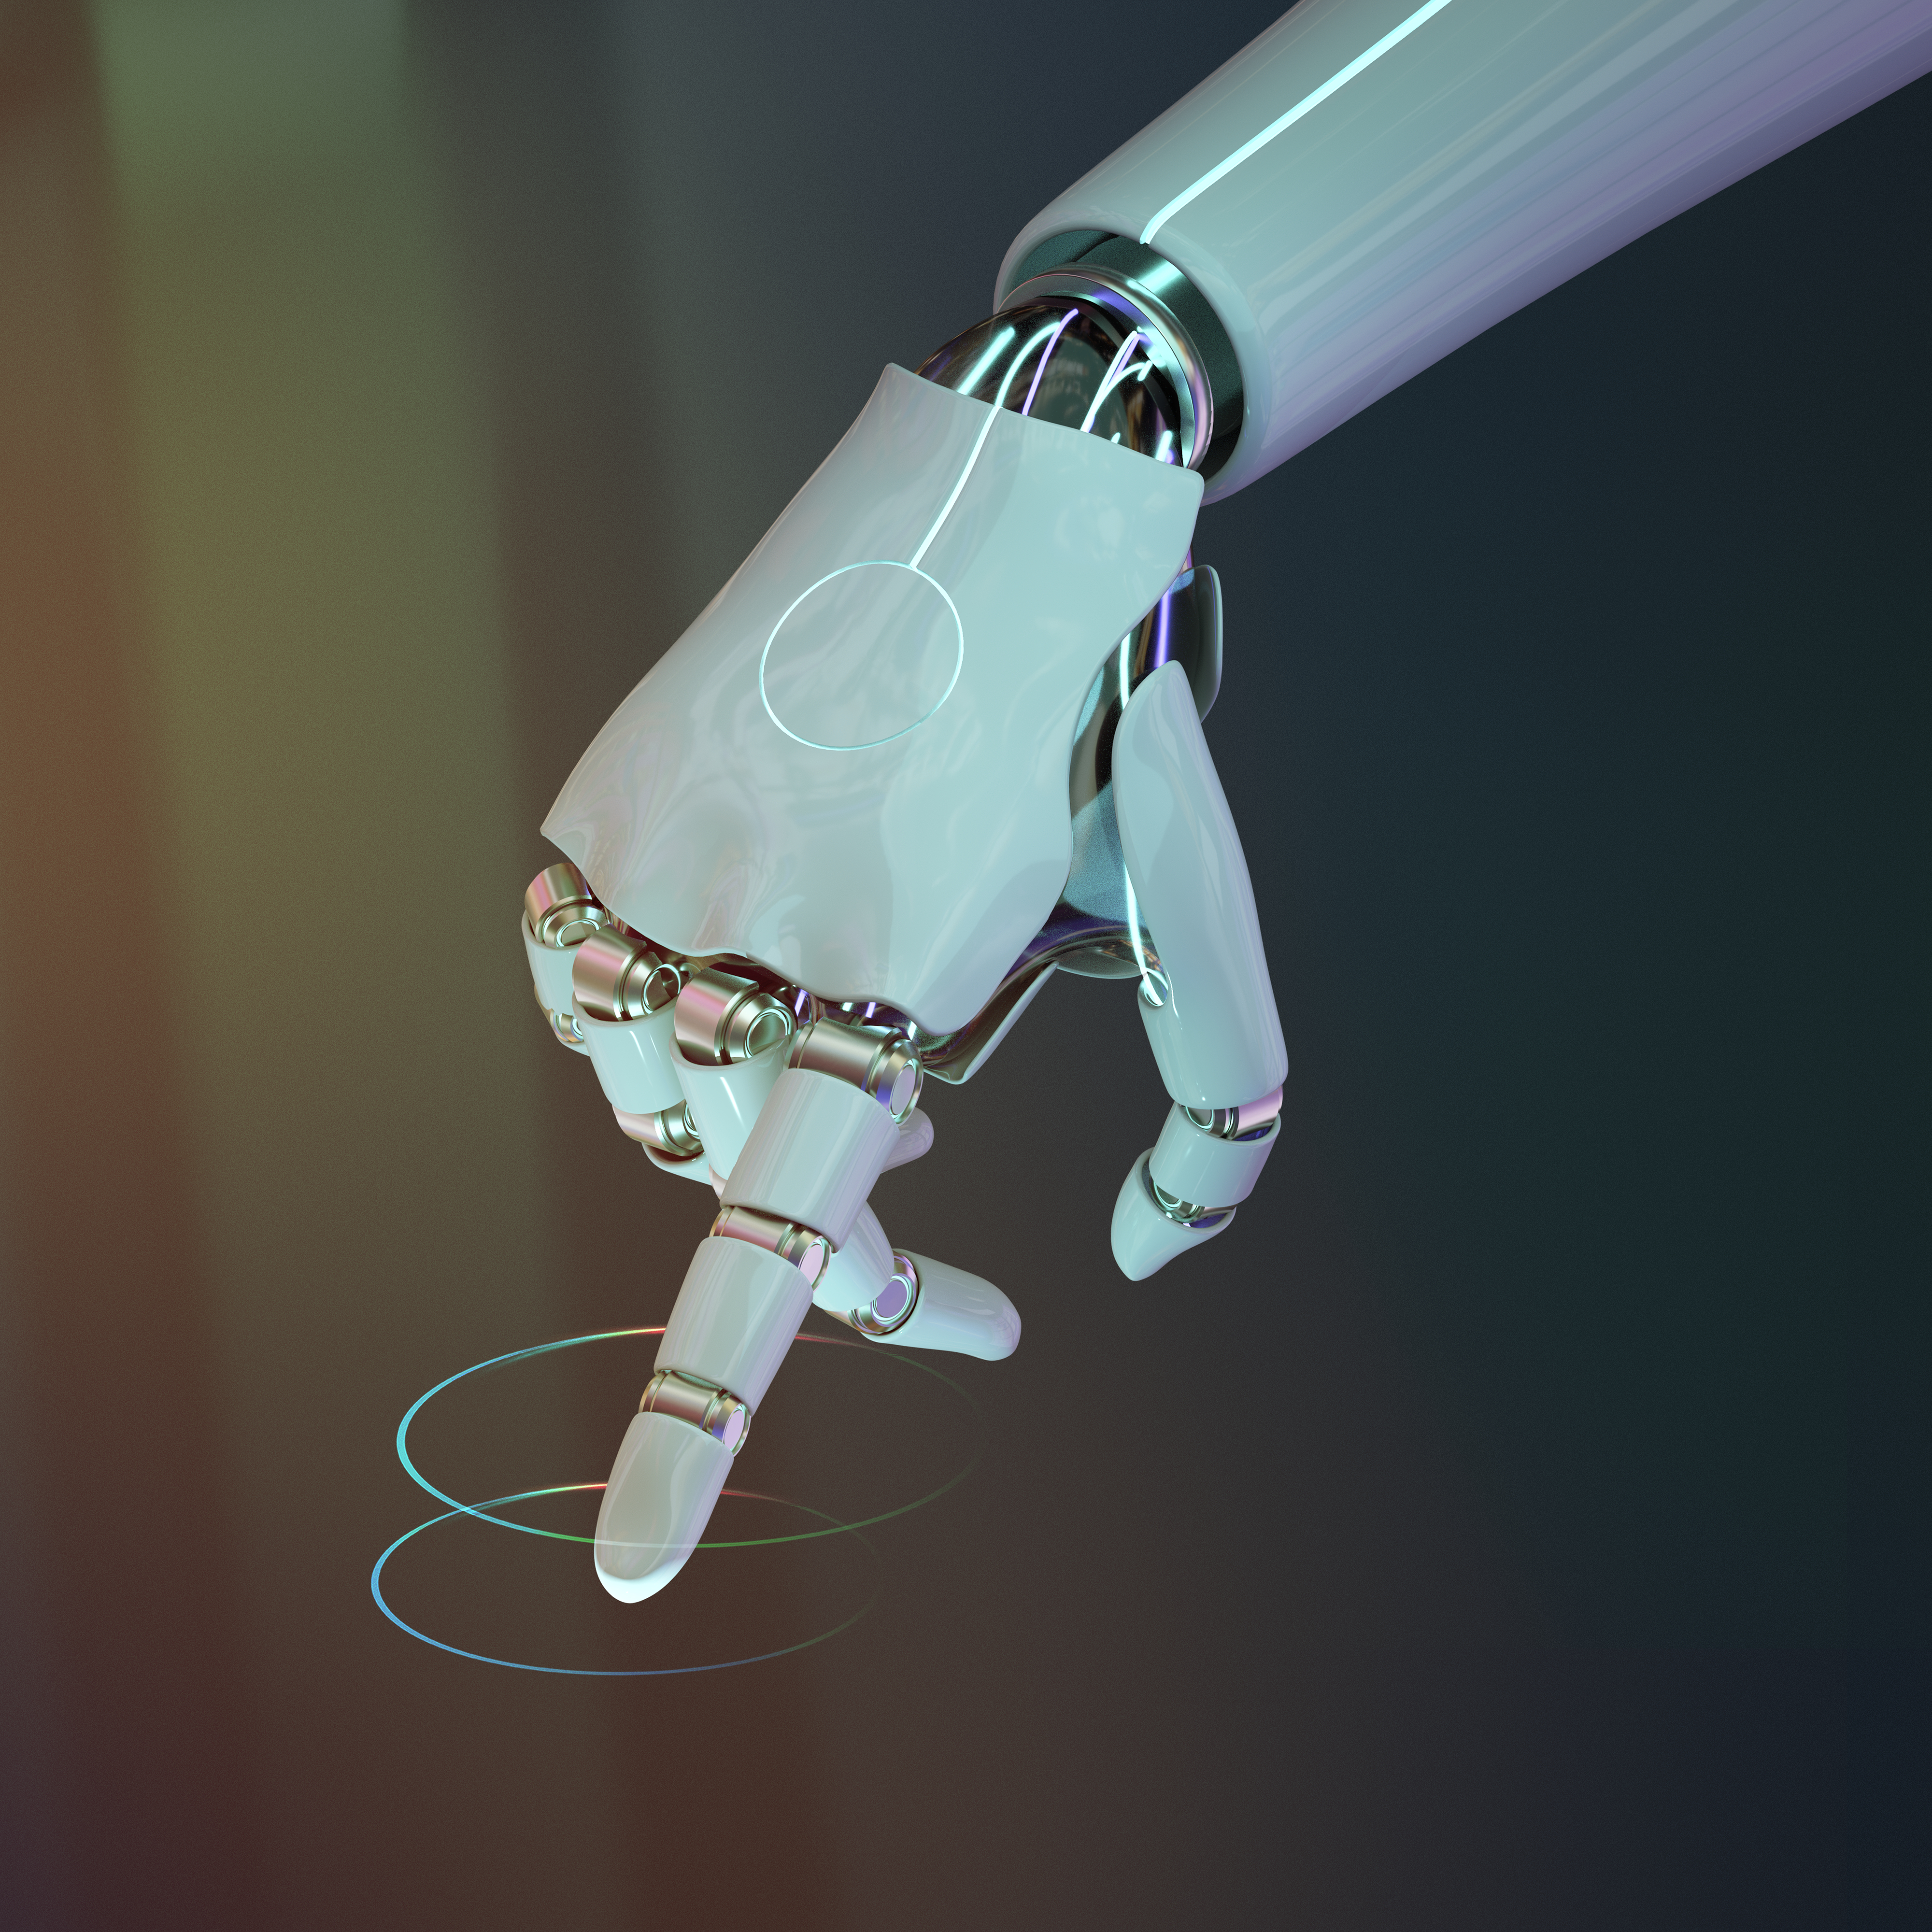
\includegraphics[width=\linewidth]{images/avenirs.jpg}
		\captionof{figure}{L’avenir de l'IA générative}
	\end{minipage}
\end{center}

\section{Comment fonctionne l'IA générative ?}
\paragraph{}
Comme toutes les intelligences artificielles, l’IA générative fonctionne en
utilisant des modèles de machine learning, de très grands modèles pré-entraînés sur
de vastes quantités de données.

\subsubsection*{Modèles de fondation}
Les modèles de fondation (FM) sont des modèles de ML entraînés sur un large éventail
de données généralisées et non étiquetées. Ils sont capables d’effectuer une
grande variété de tâches générales.

Les FM sont le résultat des dernières avancées d'une technologie qui évolue
depuis des décennies. En général, un FM utilise des modèles et des relations
appris pour prédire le prochain élément d'une séquence.

Par exemple, lors de la génération d'images, le modèle analyse l'image et crée
une version plus nette et plus clairement définie de l'image. De même, dans le
cas du texte, le modèle prédit le mot suivant dans une chaîne de texte en fonction
des mots précédents et de leur contexte. Il sélectionne ensuite le mot suivant à
l'aide de techniques de distribution de probabilité.

\subsubsection*{Grands modèles de langage}
Les grands modèles de langage (LLM) sont une classe de FM. Par exemple, les
modèles transformeurs génératifs pré-entraînés (GPT) d'OpenAI sont des LLM. Les LLM
sont spécifiquement axés sur les tâches basées sur le langage, telles que le
résumé, la génération de texte, la classification, la conversation ouverte et l'extraction
d'informations.

Ce qui rend les LLM spéciaux, c'est leur capacité à effectuer de multiples
tâches. Ils peuvent le faire car ils contiennent de nombreux paramètres qui les rendent
capables d'apprendre des concepts avancés.

Un LLM comme GPT-3 peut prendre en compte des milliards de paramètres et générer
du contenu à partir de très peu d'entrées. Grâce à leur exposition, avant l'entraînement,
à des données à l'échelle de l'Internet sous toutes leurs formes et dans une
myriade de modèles, les LLM apprennent à appliquer leurs connaissances dans un large
éventail de contextes.
\section{Fonctionnement des modèles d'IA générative}
\paragraph{}
Les modèles de machine learning traditionnels étaient discriminants ou centrés sur
la classification des points de données. Ils tentent de déterminer la relation
entre les facteurs connus et inconnus. Par exemple, ils examinent des images (des
données connues telles que la disposition des pixels, les lignes, les couleurs et
les formes) et les mappent avec des mots, le facteur inconnu. Mathématiquement
parlant, ces modèles identifient des équations qui peuvent mapper numériquement des
facteurs inconnus et connus sous forme de variables $x$ et $y$.

\paragraph{}
Les modèles génératifs vont un peu plus loin. Au lieu de prédire une étiquette en
fonction de fonctionnalités, ils essaient de prédire les caractéristiques
associées à une étiquette donnée. Mathématiquement parlant, la modélisation
générative calcule la probabilité que $x$ et $y$ apparaissent ensemble. Elle apprend
la distribution des différentes fonctionnalités des données et leurs relations.

\paragraph{}
Par exemple, les modèles génératifs analysent des images d'animaux pour enregistrer
des variables telles que différentes formes d'oreilles, d'yeux, de queue et de peau.
Ils apprennent leurs fonctionnalités et leurs relations pour comprendre à quoi
ressemblent les différents animaux en général. Ils peuvent ensuite reconstituer des
images d'animaux qui ne figuraient pas dans le jeu de données d'entraînement.

\paragraph{}
Nous allons maintenant nous pencher sur les principales catégories de modèles d'IA
générative.

% --------- Premier modèle ---------
\subsection{Modèles de diffusion}
\paragraph{}
Les modèles de diffusion créent des données en apportant de manière itérative des
modifications aléatoires contrôlées à un échantillon de données initial. Ils
commencent par ajouter des modifications subtiles (bruit) et progressives aux
données d'origine. Ce bruit est soigneusement contrôlé pour garantir que les données
générées restent cohérentes et réalistes.

Après avoir ajouté du bruit sur plusieurs itérations, le modèle de diffusion
répète le processus dans le sens inverse. Le débruitage inversé supprime progressivement
le bruit pour produire un nouvel échantillon de données qui ressemble à l'original.
\vspace{1cm}
\includegraphics[width=\textwidth]{images/modelsdiffusion.jpg}
\captionof{figure}{Exemple de modèle de diffusion}
\vspace{1cm}

% --------- Deuxième modèle ---------
\subsection{Réseaux antagonistes génératifs}
\paragraph{}
Le réseau antagoniste génératif (GAN) est un autre modèle d'IA générative qui s'appuie
sur le concept du modèle de diffusion.

Les GAN fonctionnent en entraînant deux réseaux neuronaux de manière compétitive.
Le premier réseau, appelé \textit{générateur}, génère de faux échantillons de
données en ajoutant du bruit aléatoire. Le second réseau, appelé \textit{discriminateur},
essaie de faire la distinction entre les données réelles et les fausses données
produites par le générateur.

Pendant l'entraînement, le générateur améliore continuellement sa capacité à créer
des données réalistes, tandis que le discriminateur sait de mieux en mieux
distinguer le vrai du faux. Ce processus contradictoire se poursuit jusqu'à ce que
le générateur produise des données si convaincantes que le discriminateur ne peut
pas les différencier des données réelles.

Les GAN sont largement utilisés pour la génération d'images réalistes, le
transfert de style et les tâches d'augmentation des données.

\vspace{1cm}
\includegraphics[width=\textwidth]{images/gan-datascientest-1024x512.png}
\captionof{figure}{GAN (réseaux antagonistes génératifs)}
\vspace{1cm}

% --------- Troisième modèle ---------
\subsection{Autoencodeurs variationnels}
\paragraph{}
Les autoencodeurs variationnels (VAE) apprennent une représentation compacte des
données appelée \textit{espace latent}. L'espace latent est une représentation
mathématique des données. Vous pouvez le voir comme un code unique représentant les
données en fonction de tous leurs attributs. Par exemple, si vous étudiez des visages,
l'espace latent contient des nombres représentant la forme des yeux, du nez, des
pommettes et des oreilles.

Les VAE utilisent deux réseaux neuronaux : l’\textit{encodeur} et le \textit{décodeur}.
L'encodeur mappe les données d'entrée selon une moyenne et une variance pour
chaque dimension de l'espace latent. Il génère un échantillon aléatoire à partir
d'une distribution gaussienne (normale). Cet échantillon est un point dans l'espace
latent et représente une version compressée et simplifiée des données d'entrée.

Le décodeur extrait ce point échantillonné de l'espace latent et le reconstruit
en données qui ressemblent à l'entrée d'origine. Des fonctions mathématiques sont
utilisées pour mesurer à quel point les données reconstruites correspondent aux données
d'origine.

\vspace{1cm}
\includegraphics[width=\textwidth]{images/clipseg_architecture-1.png}
\captionof{figure}{Exemple d'autoencodeur variationnel (VAE)}
\vspace{1cm}

% --------- Quatrième modèle ---------
\subsection{Modèles basés sur des transformateurs}
\paragraph{}
Les modèles d'IA générative basés sur des transformateurs s'appuient sur les concepts
d'encodeur et de décodeur des VAE. Les modèles basés sur des transformateurs
ajoutent des couches supplémentaires à l'encodeur afin d'améliorer les
performances des tâches basées sur du texte telles que la compréhension, la traduction
et l'écriture créative.

\paragraph{}
Les modèles basés sur des transformateurs utilisent un mécanisme d'\textit{auto-attention}.
Ils évaluent l'importance des différentes parties d'une séquence d'entrée lors
du traitement de chaque élément de la séquence.

\paragraph{}
Une autre fonctionnalité clé est que ces modèles d’IA implémentent des \textit{intégrations
contextuelles}. Le codage d'un élément de séquence dépend non seulement de l'élément
lui-même, mais également de son contexte dans la séquence.

\paragraph{Fonctionnement des modèles basés sur des transformeurs}
Pour comprendre le fonctionnement des modèles basés sur des transformeurs,
imaginez une phrase sous la forme d’une séquence de mots.

L'\textit{auto-attention} aide le modèle à se concentrer sur les mots pertinents
lorsqu'il traite chaque mot. Pour capturer différents types de relations entre
les mots, les modèles génératifs basés sur des transformeurs utilisent plusieurs
couches d’encodeur appelées \textit{têtes d’attention}. Chaque tête apprend à se
concentrer sur différentes parties de la séquence d’entrée, ce qui permet au
modèle de prendre en compte simultanément divers aspects des données.

Chaque couche affine également les intégrations contextuelles, les rendant plus informatives
et capturant tout, de la syntaxe grammaticale aux significations sémantiques
complexes.
\vspace{1cm}
\includegraphics[width=1\textwidth, height=5cm]{images/3D-Model-1-300x245.png}
\captionof{figure}{Modèle basé sur un transformateur}
\vspace{0.5cm}

\section{Quelles sont les limites de l’IA générative ?}

Malgré leurs avancées, les systèmes d’IA générative peuvent parfois produire des
informations inexactes ou trompeuses. Ils s’appuient sur des modèles et des données
sur lesquels ils ont été formés et peuvent refléter des biais ou des inexactitudes
inhérents à ces données. Les autres préoccupations liées aux données
d’entraînement incluent :

\subsection*{Sécurité}

Des problèmes de confidentialité et de sécurité des données se posent si des
données propriétaires sont utilisées pour personnaliser des modèles d’IA
générative. Des efforts doivent être déployés pour garantir que les outils d’IA générative
génèrent des réponses qui limitent l’accès non autorisé à des données propriétaires.
Des problèmes de sécurité se posent également en cas de manque de responsabilité
et de transparence dans la manière dont les modèles d’IA prennent des décisions.

\subsection*{Créativité}

Bien que l’IA générative puisse produire du contenu créatif, elle manque souvent
de véritable originalité. La créativité de l’IA est limitée par les données sur lesquelles
elle a été entraînée, ce qui donne lieu à des résultats qui peuvent sembler
répétitifs ou dérivés. La créativité humaine, qui implique une compréhension
plus approfondie et une résonance émotionnelle, reste difficile à reproduire pleinement
pour l’IA.

\subsection*{Coût}

L’entraînement et l’exécution de modèles d’IA générative nécessitent des
ressources de calcul importantes. Les modèles d’IA générative basés sur le cloud
sont plus accessibles et plus abordables que la création de nouveaux modèles à partir
de zéro.

\subsection*{Explicabilité}

En raison de leur nature complexe et opaque, les modèles d’IA générative sont souvent
considérés comme des boîtes noires. Il est difficile de comprendre comment ces
modèles aboutissent à des résultats spécifiques. Il est essentiel d’améliorer l’interprétabilité
et la transparence pour renforcer la confiance et l’adoption.

\section{Quelles sont les bonnes pratiques en matière d'adoption de l'IA
générative ?}

Si votre entreprise souhaite implémenter des solutions d'IA générative, tenez compte
des bonnes pratiques suivantes pour appuyer les efforts mis en œuvre.

\subsection*{Commencez par les applications internes}

Il est préférable de commencer l'adoption de l'IA générative par le
développement d'applications internes, en mettant l'accent sur l'optimisation des
processus et la productivité des employés. Vous bénéficiez d'un environnement
plus contrôlé pour tester les résultats tout en développant les compétences et
la compréhension de la technologie. Vous pouvez tester les modèles de manière approfondie
et même les personnaliser sur des sources de connaissances internes. Ainsi, vos clients
bénéficieront d’une bien meilleure expérience lorsque vous utiliserez les modèles
pour des applications externes.

\subsection*{Améliorez la transparence}

Expliquez clairement comment fonctionnent toutes les applications et tous les
résultats de l’IA générative, afin que vos utilisateurs sachent qu’ils interagissent
avec l’IA et non avec des humains. Par exemple, l'IA peut se présenter comme étant
une IA, ou les résultats de recherche basés sur l'IA peuvent être marqués et mis
en évidence. Ainsi, vos utilisateurs peuvent prendre des décisions éclairées
lorsqu'ils interagissent avec le contenu. Ils peuvent également être plus proactifs
dans le traitement des inexactitudes ou des biais cachés que les modèles sous-jacents
peuvent présenter en raison des limites de leurs données d'apprentissage.

\subsection*{Implémentez la sécurité}

Mettez en place des barrières de protection permettant à vos applications d'IA
générative de refuser l'accès non autorisé aux données sensibles. Impliquez les équipes
de sécurité dès le départ afin que tous les aspects puissent être pris en compte
immédiatement. Par exemple, vous devrez peut-être masquer des données et supprimer
des données d'identification personnelle (PII) avant d'entraîner des modèles sur
des données internes.

\subsection*{Effectuez des tests exhaustifs}

Développez des processus de test automatisés et manuels pour valider les
résultats et testez tous les types de scénarios auxquels le système d’IA
générative peut être confronté. Formez plusieurs groupes de bêta-testeurs pour essayer
les applications de différentes manières et documenter les résultats. Le modèle
s'améliorera également en continu grâce aux tests, et vous aurez un meilleur contrôle
sur les résultats attendus et les réponses.

\section{Amélioration de la pertinence des chatbots d'IA générative}
\section*{Qu’est-ce qu’un modèle pré-entraîné ?}

Quand on parle de modèles d’IA, on parle généralement d’algorithmes utilisant des
réseaux de neurones. Cette technologie est utilisée par les \textit{Larges
Modèles de Langage} (LLM) comme \textit{ChatGPT} ou \textit{Mistral Large}, par
les algorithmes de génération d’images ou de reconnaissance visuelle. Ces modèles
sont entraînés sur des jeux de données très volumineux, leur permettant
d’acquérir une base solide dans le domaine de compétences qu’ils vont maîtriser.

Il est possible de régler de nombreux paramètres sur les différentes couches
d’un réseau pour modifier la manière dont est traitée l’information. On arrive à
plusieurs milliards de paramètres lorsque les modèles sont vraiment volumineux (de
quoi laisser de la place à la personnalisation\ldots) !

\subsection{RAG (Retrieval-Augmented Generation)}
\paragraph{}
Le \textit{Retrieval Augmented Generation} (RAG) est une approche novatrice qui combine
le meilleur de deux mondes en IA : la recherche d’informations (\textit{retrieval},
qui ne génère pas de réponse originale) et la génération de contenu (qui ne
s’appuie que sur les données de son entraînement).

Traditionnellement, les \textit{Large Language Models} (LLM) génèrent du contenu
en s’appuyant uniquement sur les informations apprises durant leur phase d’entraînement.
Le RAG, en revanche, permet au modèle de « consulter » une base de données ou un
corpus de documents externes en temps réel pour enrichir sa génération de texte.

Cette capacité de recherche améliore significativement la précision, la pertinence
et la richesse du contenu généré.

\section*{Comment fonctionne le RAG ?}

Le processus du \textit{Retrieval Augmented Generation} (RAG) peut être divisé en
deux grandes étapes :

\begin{itemize}
	\item \textbf{La récupération} : Lorsque le modèle reçoit une requête, il effectue
		une recherche dans un ensemble prédéfini de documents ou de données pour trouver
		les informations les plus pertinentes par rapport à la requête. Cette
		recherche est souvent facilitée par des techniques d’indexation et de
		récupération d’informations sophistiquées.

	\item \textbf{La génération} : Une fois les informations pertinentes
		récupérées, le modèle les utilise, en plus de sa propre connaissance interne,
		pour générer une réponse ou un contenu qui non seulement répond à la requête
		initiale mais le fait de manière plus informée et précise.
\end{itemize}
\section*{Avantages du RAG}

L’intégration du \textit{Retrieval Augmented Generation} dans les systèmes d’IA
générative offre plusieurs avantages significatifs, améliorant non seulement la qualité
du contenu généré mais aussi son applicabilité dans divers contextes.

\subsection*{Amélioration de la pertinence et de l'exactitude}
En puisant dans une base de données externe pour compléter ses connaissances, un
modèle RAG peut fournir des réponses plus précises et pertinentes aux questions
posées. Cela est particulièrement utile pour les requêtes nécessitant des données
actualisées ou spécifiques à un domaine.

\subsection*{Contenu plus riche et informé}
La génération de contenu ne se contente plus de refléter les connaissances préalablement
acquises pendant l’entraînement du modèle. Cela conduit à la création de textes
plus informatifs, détaillés et nuancés.

\subsection*{Flexibilité et adaptabilité}
Grâce à sa capacité à consulter une vaste gamme de sources, un modèle RAG peut
s’adapter à une variété de sujets et de domaines. Cette flexibilité le rend particulièrement
précieux pour les applications nécessitant une expertise dans des domaines de niche
ou en constante évolution.

\subsection*{Interactivité améliorée}
Le RAG permet aux systèmes d’interagir de manière plus sophistiquée avec les utilisateurs,
en répondant à des questions complexes ou en fournissant des explications
détaillées qui s’appuient sur des données et des sources externes.

\subsection*{Applications du RAG}

Les applications du RAG sont multiples et permettent d’améliorer grandement la qualité
du contenu généré. Voici quelques exemples illustrant comment cette approche
peut s’intégrer à différents environnements professionnels :

\begin{itemize}[leftmargin=1.5cm]
	\item \textbf{Support client} : Le RAG permet de fournir des réponses
		personnalisées et précises aux requêtes des clients en accédant en temps
		réel à une base de données exhaustive, améliorant ainsi l’expérience client.
		Les systèmes de support équipés de RAG peuvent générer des FAQ dynamiques, répondant
		aux questions courantes avec des informations à jour, réduisant le volume de
		requêtes nécessitant une intervention humaine.

	\item \textbf{Génération de contenu} : Dans le marketing, le RAG peut être utilisé
		pour créer des articles, des billets de blog, et des descriptions de produits
		personnalisés pour le public cible, en s’appuyant sur des données de
		recherche pertinentes.

	\item \textbf{Ventes} : Le RAG peut dynamiser les stratégies de vente en
		créant des propositions commerciales sur mesure qui résonnent avec les
		besoins et préférences spécifiques des prospects. Basé sur l’analyse des interactions
		précédentes avec un client, le modèle peut générer des scripts de vente
		optimisés et des points de discussion pertinents.

	\item \textbf{Ressources humaines} : Le RAG facilite la rédaction de
		descriptions de poste attractives et précises, en s’inspirant des meilleures
		pratiques et des exemples de succès dans l’industrie. Il permet également de
		créer des FAQ internes détaillées, répondant efficacement aux questions des employés
		en se référant à des politiques et procédures actualisées, favorisant ainsi
		un environnement de travail informé et harmonieux.
\end{itemize}

\subsection*{Défis et limites}

Malgré ses nombreux avantages, le RAG n’est pas sans défis. La qualité et la pertinence
des informations récupérées dépendent fortement de la qualité du corpus de documents
sous-jacent. De plus, l’intégration efficace des informations récupérées dans la
génération de texte reste un défi technique non négligeable. Enfin, des considérations
éthiques et de confidentialité entrent en jeu lorsqu’il s’agit de déterminer quelles
informations peuvent être récupérées et utilisées par ces modèles.

\subsection{Fine-Tuning ?}
Contrairement à l’entraînement initial qui nécessite des jeux de données massifs
comme ImageNet, cet affinage se concentre sur des données plus restreintes et
spécialisées.

Il s’agit d’un processus itératif qui vise à améliorer la performance du modèle
sur une tâche particulière, sans perdre les connaissances préalables acquises lors
de l’entraînement initial.

L’idée centrale réside dans la capacité du modèle à généraliser à de nouveaux domaines
tout en conservant sa capacité à se spécialiser.

Cette approche trouve des applications variées à travers de nombreux domaines comme
:
\begin{itemize}
	\item \textbf{Computer Vision} : un modèle peut être fine-tuné pour la
		détection d’objets spécifiques dans des contextes particuliers (véhicules autonomes,
		caméras de surveillance).

	\item \textbf{Médical} : un modèle peut être affiné pour la détection
		d’organes spécifiques dans les images médicales.

	\item \textbf{NLP} : un modèle peut être adapté pour la classification de
		documents juridiques, la détection de tonalité émotionnelle, ou la
		traduction automatique spécialisée.
\end{itemize}

\subsection*{Les étapes du processus de Fine-Tuning}
Le Fine-Tuning suit une approche méthodique :
\begin{enumerate}
	\item \textbf{Collecte et préparation des données} : données spécifiques, de haute
		qualité, nettoyées.

	\item \textbf{Choix du modèle pré-entraîné} selon la tâche cible.

	\item \textbf{Évaluation initiale} du modèle sur la tâche cible pour disposer
		d'une base de référence.

	\item \textbf{Ajustement des hyperparamètres} (taux d’apprentissage, nombre
		d’itérations, taille du lot).
\end{enumerate}

Pour optimiser ces hyperparamètres, on peut utiliser :
\begin{itemize}
	\item la recherche aléatoire,

	\item la recherche en grille,

	\item l’optimisation bayésienne.
\end{itemize}

\subsection*{Les stratégies avancées d’affinage}
Au-delà du simple ajustement, plusieurs stratégies avancées existent :
\begin{itemize}
	\item \textbf{Transfert d’apprentissage} : utiliser la connaissance acquise
		sur une tâche pour une autre tâche similaire.

	\item \textbf{Fine-Tuning progressif} : affiner progressivement, en commençant
		par les couches supérieures, puis inférieures.

	\item \textbf{Techniques de régularisation} comme le dropout pour limiter le
		surajustement.
\end{itemize}

Une évaluation à chaque étape permet de détecter signes de surajustement ou de sous-ajustement.

\subsection*{Les meilleurs outils et bibliothèques de Fine-Tuning}
Parmi les outils les plus utilisés :
\begin{itemize}
	\item \textbf{TensorFlow} : fonctionnalités avancées de transfert
		d’apprentissage.

	\item \textbf{Keras} : interface haut niveau simplifiant le Fine-Tuning.

	\item \textbf{PyTorch} : flexibilité et manipulation aisée des couches du
		modèle.

	\item \textbf{Hugging Face Transformers} : bibliothèque de modèles pré-entraînés.
\end{itemize}

Pour la visualisation :
\begin{itemize}
	\item \textbf{TensorBoard} pour TensorFlow,

	\item \textbf{TensorBoardX} pour PyTorch.
\end{itemize}

Les communautés GitHub et Stack Overflow offrent aussi de nombreux exemples,
tutoriels et solutions aux problèmes courants.

\subsection*{Les défis du Fine-Tuning : difficultés à surmonter}
Parmi les défis principaux :
\begin{itemize}
	\item \textbf{Surajustement} : atténué par des techniques comme le dropout ou
		la normalisation par lots.

	\item \textbf{Déséquilibre des classes} : l’usage de poids de classe peut
		corriger ce biais.

	\item \textbf{Amplification des biais} : diversifier les sources de données et
		utiliser des techniques de correction de biais.
\end{itemize}
\subsection{Le prompt engineering }

Le prompt engineering, aussi appelé « ingénierie de requête », est une technique
qui consiste à fournir des instructions détaillées aux modèles de traitement du langage
naturel (Natural Language Processing, ou NLP) afin d’améliorer leurs
performances.

Concrètement, le prompt engineering permet de guider plus précisément un modèle NLP
en lui donnant des indications sur la tâche à effectuer et le contexte dans lequel
elle s’inscrit. Plutôt que de laisser le modèle répondre de manière générique à
une question posée, le prompt engineering permet de cadrer la réponse attendue.

Par exemple, il est possible d’utiliser le prompt engineering pour entraîner un
modèle de génération de texte à rédiger des e-mails de relance client plus
efficaces et personnalisés. Au lieu de lui donner comme simple instruction « Rédigez
un e-mail de relance client », le prompt engineering doit fournir des détails :
« Rédigez un e-mail de 200 mots pour relancer le client Jean Dupont qui n’a pas
payé sa dernière facture depuis 30 jours. Utilisez un ton courtois et proposez une
remise de 10\% s’il paie dans les 7 prochains jours. »

Ainsi, le prompt engineering permet de mieux contrôler et orienter les réponses d’un
modèle NLP en fournissant un contexte, des exemples et des instructions claires.

\subsection*{Comment fonctionne le prompt engineering ?}

L’utilisation du prompt engineering repose sur deux mécanismes complémentaires.
D’une part, l’entraînement via des exemples commentés : cette technique consiste
à fournir au modèle NLP des exemples concrets de prompts efficaces, accompagnés
d’explications sur les raisons qui les rendent performants. Par exemple, les
prompts donnés au modèle peuvent être conçus pour générer des slogans
publicitaires impactants, en expliquant pourquoi ils cadrent bien la tâche attendue.

D’autre part, l’orientation pas à pas : le modèle est guidé étape par étape sur
la façon de construire un prompt optimal. Il est, par exemple, possible de lui indiquer
qu’un bon prompt doit définir clairement l’objectif, donner des exemples
pertinents, établir le contexte, utiliser un vocabulaire simple, etc.

En combinant ces deux techniques, le modèle « apprend » à générer de meilleurs
prompts de manière autonome. À force d’exemples commentés et d’orientation, le
modèle finit par intégrer les bonnes pratiques du prompt engineering et les
appliquer de lui-même.

L’enjeu est de fournir suffisamment d’informations dans le prompt pour que le
modèle produise une réponse de qualité, mais sans non plus le surcharger d’instructions
qui limitent sa créativité. Le prompt engineering cherche ainsi le bon équilibre
entre guidage et autonomie.

\subsection*{Quels sont les différents types de prompt engineering ?}

Il existe plusieurs façons d’aborder le prompt engineering en fonction du résultat
recherché. Voici les trois grands types de prompt engineering :

\begin{itemize}
	\item Le prompt engineering pour l’entraînement des modèles : il consiste à fournir
		au modèle NLP des prompts spécifiquement conçus pour l’entraîner sur une tâche
		donnée. Par exemple, lui donner des milliers de prompts illustrant la génération
		de textes publicitaires.

	\item Le prompt engineering pour l’inférence en production : une fois le modèle
		déployé, il est alimenté avec des prompts optimisés pour les cas d’usage
		visés. Cette méthode est utilisée pour les prompts de modération de contenu,
		de réponse aux questions clients, etc.

	\item Le prompt engineering adaptatif : le modèle NLP est entraîné à générer lui-même
		les meilleurs prompts en fonction du contexte. Cette approche a pour but de
		rendre le modèle capable d’un prompt engineering autonome.
\end{itemize}

Chacune de ces variantes présente des spécificités en termes de méthodologie. Le
prompt engineering pour l’entraînement met l’accent sur la diversité et la quantité
de données. Celui pour l’inférence se concentre sur la qualité des prompts en
contexte réel. L’approche adaptative cherche à donner au modèle la capacité d’apprendre
à faire un prompt engineering efficace par lui-même.

Les chercheurs combinent souvent ces différents types de prompt engineering de manière
complémentaire pour obtenir les meilleures performances. Cette diversité des
techniques de prompt engineering est une force pour cette discipline encore
émergente.

\subsection*{Quelles compétences requiert la maîtrise du prompt engineering ?}

Réussir dans le prompt engineering, sans pour autant être un prompt engineer (ingénieur
de requête), requiert de solides compétences pluridisciplinaires.

Tout d’abord, une connaissance approfondie des modèles de traitement du langage
naturel est indispensable pour créer des prompts adaptés à leurs forces et à
leurs limites.

La rédaction est également cruciale, car le prompt se doit d’être un texte concis,
précis et cohérent. De bonnes capacités rédactionnelles sont donc essentielles.

La maîtrise de techniques d’apprentissage automatique comme le transfer learning
est aussi un atout, celles-ci étant souvent employées conjointement au prompt
engineering.

De même, une expertise en linguistique computationnelle permet de mieux appréhender
les mécanismes d’interprétation du langage par les modèles.

Côté technique, la programmation et la data science sont nécessaires pour
intégrer et évaluer les performances des prompts. La rigueur dans les tests et les
expérimentations permet d’identifier les prompts les plus efficaces.

Enfin, la créativité et un esprit critique sont des qualités essentielles pour
le prompt engineering.

\subsection*{Quels sont les avantages du prompt engineering ?}

L’utilisation du prompt engineering présente plusieurs avantages. Tout d’abord, cette
technique permet d’obtenir des réponses plus précises et pertinentes de la part des
modèles NLP. Avec un prompt bien conçu, le modèle va générer une réponse correspondant
exactement à la tâche demandée, et non pas quelque chose de vague ou
d’approximatif.

Le prompt engineering assure également une meilleure adéquation entre la réponse
du modèle et les besoins spécifiques de l’utilisateur, en cadrant la génération de
texte en fonction du cas d’usage visé et des instructions fournies. Par ailleurs,
un prompt détaillé va limiter les contresens et mauvaises interprétations du modèle
NLP, réduisant ainsi les biais et les erreurs. Le prompt engineering favorise aussi
une plus grande cohérence des réponses du modèle, même face à des inputs
différents.

À terme, cette technique améliore les performances globales des modèles NLP en renforçant
leur capacité à comprendre des demandes complexes. Enfin, le prompt engineering offre
une meilleure contrôlabilité de ces modèles, en permettant à leurs concepteurs
d’orienter finement leur comportement via les consignes fournies.

\subsection*{Quelles sont les limites du prompt engineering ?}

Bien que présentant des avantages certains, l’utilisation du prompt engineering
comporte également des limites qu’il faut garder à l’esprit. Tout d’abord, il
s’agit d’une technique qui nécessite un investissement temps important ainsi que
de solides compétences en conception de prompts pour élaborer des instructions
optimales. Sans une expertise approfondie, il est assez facile de rédiger de
mauvais prompts qui vont en réalité dégrader les performances du modèle NLP au
lieu de les améliorer.

De plus, le prompt engineering est fortement dépendant du cas d’usage : des prompts
spécifiques à une tâche devront être entièrement réécrits en cas de changement d’objectif
ou de contexte. Par ailleurs, des prompts trop directifs ou détaillés peuvent réduire
la créativité et l’autonomie des modèles NLP en les enfermant dans des schémas de
réponse prédéfinis et stéréotypés. L’équilibre subtil entre guidage et liberté
accordée au modèle est difficile à trouver.

Le processus de conception de prompts efficaces s’appuie également sur de
nombreux essais-erreurs, des ajustements progressifs et de fins réglages : un prompt
optimal ne peut être obtenu immédiatement.

Enfin, la complexité des prompts tend à croître à mesure qu’on cherche à les
optimiser, jusqu’à potentiellement devenir contre-productifs s’ils sont surchargés
d’instructions. Malgré son potentiel prometteur, le prompt engineering ne constitue
donc pas une solution magique aux limitations des modèles NLP actuels.

\subsection*{Comment le prompt engineering va-t-il évoluer ?}

Même s’il s’agit d’une technologie déjà mature, le prompt engineering devrait encore
progresser à l’avenir, notamment grâce aux avancées dans les domaines connexes
du transfer learning et du few-shot learning.

Plusieurs évolutions sont à anticiper :

\begin{itemize}
	\item L’émergence de nouvelles méthodes pour générer des prompts plus efficaces,
		via l’utilisation d’algorithmes d’optimisation par exemple ;

	\item Le développement de bibliothèques de prompts pré-écrits, réutilisables
		d’un modèle NLP à l’autre ;

	\item La possibilité pour les modèles d’auto-générer les prompts les plus adaptés
		en fonction de la tâche demandée ;

	\item L’utilisation du prompt engineering pour entraîner des modèles NLP toujours
		plus puissants, atteignant des niveaux de compétence linguistique proches de
		l’humain ;

	\item L’écriture de prompts par les utilisateurs finaux eux-mêmes, permettant
		de guider les modèles NLP en langage naturel ;

	\item Une intégration accrue entre prompt engineering et techniques de search.
\end{itemize}

Grâce à ces avancées, le prompt engineering a le potentiel de devenir une technique
incontournable pour exploiter au maximum les capacités des modèles de traitement
du langage naturel sur une grande diversité de cas d’usage.

\subsection{Few Shot Learning ?}
Le Few Shot Learning (FSL) est un framework du domaine du Machine Learning,
c’est-à-dire une structure de base pour le développement de codes de
programmation. Il est utilisé pour entraîner les modèles d’IA à faire des prédictions
précises à partir d’une petite quantité de données d’entraînement. Alors que les
méthodes de Machine Learning traditionnelles nécessitent souvent des milliers de
points de données pour fournir des résultats fiables, le Few Shot Learning vise à
optimiser l’apprentissage avec un minimum de données.

L’objectif principal du Few Shot Learning est un apprentissage efficace à partir
de quelques exemples seulement. En travaillant avec une quantité minimale de
données, le FSL s’avère particulièrement utile dans les situations où il est difficile
de collecter de grandes quantités de données étiquetées (ex : maladies rares, manuscrits
uniques).

Le Few Shot Learning peut être considéré comme un sous-groupe du n-Shot-Learning
(N-Way-K-Shot), où : - $N$ est le nombre de classes, - $K$ est le nombre
d’exemples par classe.

Cela comprend également : - le One Shot Learning (un exemple par classe), - le Zero
Shot Learning (aucun exemple étiqueté).

\subsection*{Comment fonctionne le Few Shot Learning ?}
Même si des algorithmes spéciaux et des réseaux neuronaux réussissent de nombreuses
tâches de FSL, il est avant tout défini par le **problème d’apprentissage**
spécifique, et non par un modèle particulier.

Les principales approches sont :

\subsubsection*{Apprentissage par transfert}
Il s'agit d'adapter des modèles pré-entraînés pour de nouvelles tâches, en utilisant
les connaissances déjà acquises pour éviter le surajustement, surtout avec peu d'exemples.
Cela fonctionne particulièrement bien si la tâche cible est similaire à la tâche
d’origine.

\subsubsection*{Approche par les données}
Il s'agit de **générer des données supplémentaires** pour pallier le manque d'exemples,
souvent grâce à des réseaux génératifs (GANs). Cela est crucial dans des cas rares
(ex : espèces nouvellement découvertes).

\subsubsection*{Meta Learning (Méta-apprentissage)}
Le modèle apprend à apprendre : il généralise des schémas à travers différentes tâches.

On distingue deux types :

\paragraph*{Méta-apprentissage basé sur les métriques}
Plutôt que de modéliser des classes directement, on apprend des distances entre
exemples : - Réseaux siamois - Réseaux de matching - Réseaux prototypiques -
Réseaux de relation (Relation Networks)

\paragraph*{Méta-apprentissage basé sur l’optimisation}
On optimise les modèles pour qu'ils s'adaptent rapidement à de nouvelles tâches
: - MAML (Model Agnostic Meta-Learning) - Optimisation par LSTM - LEO (Latent Embedding
Optimization)

\subsection*{Principaux domaines d’application du Few Shot Learning}
Les secteurs concernés sont nombreux :

\begin{itemize}
	\item \textbf{Computer Vision} : classification d’images, reconnaissance d’objets.

	\item \textbf{Robotique} : adaptation rapide à de nouveaux environnements.

	\item \textbf{Traitement du langage} : adaptation de grands modèles de langage.

	\item \textbf{Santé publique} : diagnostic de maladies rares.

	\item \textbf{Secteur bancaire} : détection de fraudes avec peu d’exemples.
\end{itemize}

\subsection*{Enjeux concrets liés à la mise en œuvre du Few Shot Learning}
Le Few Shot Learning présente plusieurs défis :
\begin{itemize}
	\item \textbf{Surajustement} : le risque est élevé avec peu de données.

	\item \textbf{Qualité des données} : si les données sont de mauvaise qualité, la
		performance chute.

	\item \textbf{Sélection de caractéristiques} : difficile avec peu d’exemples.

	\item \textbf{Ressources de calcul} : optimisation fine requiert du temps et
		des ressources.
\end{itemize}

\subsection{Low Rank Adaptation}
Cette approche novatrice se concentre sur la réduction de la dimensionnalité des
données, dans le but de faciliter l’adaptation de domaine : le transfert d’un modèle
depuis un domaine source où il est entraîné vers un domaine cible où les données
peuvent être différentes.

Un concept central de cette méthode est la décomposition à faible rang des matrices.
Celle-ci permet de représenter les données sous une forme plus compacte, tout en
préservant leur structure sous-jacente.

Dans le contexte de l’apprentissage automatique, cette décomposition vise à
extraire les caractéristiques les plus importantes des données d’entraînement. Le
but est de construire un modèle plus généralisable pour le domaine cible.

Il existe différentes méthodes pour y parvenir. Les plus utilisées sont la
décomposition en valeurs singulières (Singular Value Decomposition ou SVD) et la
décomposition en facteurs non négatifs (Non-Negative Matrix Factorization ou NMF).

Grâce à la réduction de dimensionnalité des données, on évite les problèmes de surajustement
(overfitting) pouvant survenir quand les modèles sont directement appliqués à des
données de cibles différentes. C’est ce qui simplifie le transfert de
connaissances.

L’un des principaux points forts de la Low Rank Adaptation est sa capacité à
capturer les corrélations et dépendances entre les caractéristiques des données.
Ainsi, l’information cruciale pour l’adaptation est mieux représentée.

Un autre avantage est la possibilité d’appliquer cette approche à différentes
tâches de Machine Learning comme la classification, la régression ou même la génération
de données synthétiques.

\subsection*{À quoi ça sert ? Quelles sont les applications ?}
La Low Rank Adaptation est une méthode qui a fait ses preuves, et qui est déjà
adoptée dans de nombreux domaines du Machine Learning.

Dans la vision par ordinateur (Computer Vision), elle est utilisée pour la reconnaissance
d’objets au sein d’environnements différents de ceux utilisés pour l’entraînement
initial.

En utilisant des décompositions à faible rang sur les représentations des caractéristiques
des images, les modèles ML peuvent mieux généraliser à de nouvelles conditions
d’éclairage, d’angle de vue ou d’environnement pour améliorer considérablement leurs
performances dans le monde réel.

Pour le NLP ou traitement naturel du langage, cette approche s’avère aussi très
efficace pour les tâches de traduction automatique.

Alors que les données des domaines sources et cibles peuvent considérablement
varier, l’adaptation à faible rang permet de créer des modèles plus flexibles en
extrayant les aspects linguistiques essentiels et en les appliquant au nouveau domaine.
La traduction dans des contextes différents s’en trouve améliorée.

De même, pour la reconnaissance de la parole, la Low Rank Adaptation est utile
pour adapter les modèles de reconnaissance vocale à des locuteurs spécifiques ou
à différents environnements acoustiques.

Les techniques de décomposition à faible rang permettent aux systèmes de mieux
capturer les variations entre les interlocuteurs et donc d’obtenir une meilleure
précision dans des situations variées.

Enfin, en intégrant cette méthode d’adaptation aux architectures de réseaux de neurones,
l’apprentissage par transfert est facilité. Les connaissances acquises dans un domaine
sont transmises à un domaine cible, augmentant fortement les performances pour
une large variété de tâches.

\subsection*{Les défis de la Low Rank Adaptation}
Tous les exemples évoqués dans le chapitre précédent démontrent l’efficacité de
la Low Rank Adaptation pour surmonter les défis liés à l’adaptation de domaine
dans le Machine Learning.

Malgré ses nombreux avantages, cette approche présente aussi des défis spécifiques
à relever. Par exemple, la gestion du surajustement (overfitting) et du sous-ajustement
(underfitting) des modèles peut être difficile.

Une décomposition à faible rang trop restrictive peut entraîner une perte d’informations
cruciales, tandis qu’une décomposition trop complexe peut conduire à la
suradaptation aux données d’entraînement. Trouver le bon équilibre est donc essentiel
pour l’optimisation des performances sur de nouvelles données.

Autre problème potentiel : les domaines sources et cibles peuvent être extrêmement
différents, ce qui entraîne une hétérogénéité des données compliquant fortement
l’adaptation.

La diversité des caractéristiques entre les deux domaines peut en effet affecter
la capacité du modèle à transférer des connaissances de manière appropriée.

Pour éviter ce désagrément, il convient de développer des techniques de décomposition
à faible rang capables de capturer les variations tout en conservant les structures
essentielles.

Enfin, dans de nombreuses situations, il n’est pas toujours évident d’obtenir des
données étiquetées dans le domaine cible. Elles peuvent être limitées, ou tout simplement
trop coûteuses.

Or, la Low Rank Adaptation requiert généralement une large quantité de données
pour construire des modèles généralisables. Ceci exige des recherches supplémentaires
pour développer des méthodes exploitant les données non étiquetées ou semi-étiquetées,
comme l’adaptation à faible rang transductive.
\newpage
{}
\subsection{Comparaison des Techniques}
\begin{table}[h!]
	\caption{Comparaison des principales techniques d'optimisation de modèles d'IA}
	\centering
	\begin{tabular}{|p{3cm}|p{5cm}|p{5cm}|}
		\hline
		\textbf{Technique}                   & \textbf{Avantages}                                                                                  & \textbf{Limitations}                                                                              \\
		\hline
		RAG (Retrieval-Augmented Generation) & - Accès à des informations actualisées \newline - Améliore la pertinence des réponses               & - Dépendance aux bases de données \newline - Complexité de mise en œuvre                          \\
		\hline
		Fine-Tuning                          & - Modèle spécialisé pour une tâche précise \newline - Meilleure performance sur des cas spécifiques & - Coûteux en calculs \newline - Nécessite beaucoup de données                                     \\
		\hline
		Prompt Engineering                   & - Pas besoin de réentraîner le modèle \newline - Rapide à mettre en place                           & - Résultats instables \newline - Fortement dépendant de la qualité du prompt                      \\
		\hline
		Few-Shot Learning                    & - Apprentissage avec peu d'exemples \newline - Réduit le besoin de grandes bases de données         & - Moins performant qu'un entraînement complet \newline - Peut être sensible au choix des exemples \\
		\hline
		LoRA (Low-Rank Adaptation)           & - Fine-tuning léger \newline - Moins de ressources nécessaires                                      & - Peut être moins performant que le fine-tuning complet                                           \\
		\hline
		Distillation                         & - Modèle plus léger et rapide \newline - Adapté aux environnements contraints (mobile, embarqué)    & - Perte de performance par rapport au modèle original                                             \\
		\hline
	\end{tabular}
	\label{tab:comparaison-techniques}
\end{table}
\newpage
{}
\section*{Conclusion}
\addcontentsline{toc}{section}{Conclusion}
Dans ce chapitre, nous avons découvert l'univers fascinant de l'intelligence
artificielle générative. Cette technologie, qui permet de créer du contenu
original (textes, images, sons...), repose sur des modèles puissants comme les
autoencodeurs variationnels (VAE), les réseaux antagonistes génératifs (GAN) ou encore
les transformateurs.
\paragraph{}
Nous avons vu que l'IA générative offre énormément d'opportunités, mais qu’elle
comporte aussi des risques et des limites. Elle peut révolutionner des domaines comme
l'art, la santé ou l'éducation, tout en soulevant des questions importantes autour
de l'éthique, de la fiabilité et de l'utilisation abusive.
\paragraph{}
Grâce aux nouvelles techniques comme le fine-tuning, le prompt engineering ou le
few-shot learning, il est possible d'améliorer encore la pertinence et la
qualité des résultats produits. Mais pour en tirer le meilleur parti, il est
essentiel de l'utiliser avec précaution et de garder à l'esprit l'importance de
l'humain dans le processus.
\paragraph{}
L'IA générative n'en est qu'à ses débuts. Elle continuera d'évoluer et de transformer
notre quotidien. À nous de savoir l’accompagner de manière responsable, en restant
attentifs aux défis qu’elle pose et en utilisant son potentiel pour construire des
outils plus créatifs, plus justes et plus utiles.

%%%%%%%%%%%%%%%%%%%%%%%%%%%%%%%%%%%%%%%%%%%%%%%%%%%%%%%%%%%%%%%%%%%%%%%%%%%%%%
%%%%%%%%%%%%%%%%%%%%%%%%%%%%%%%%%%%%%%%%%%%%%%%%%%%%%%%%%%%%%%%%%%%%%%%%%%%%%%
% Chapitre 2

%%% Intro chapitre 2
\chapter{Chapitre 2 : Présentation de l'entreprise}
\section*{Introduction}
\phantomsection
\addcontentsline{toc}{section}{Introduction}
\paragraph{}
\lipsum[1]

\section{La société} 
\paragraph{}
        \subsection{Les activités}
        \paragraph{}
        \subsection{Les services}
        \paragraph{}
        \subsection{Les produits}
        \paragraph{}
        \subsection{Les clients}
        \paragraph{}
        \subsection{Les partenaires}
        \paragraph{}
        \subsection{Les ressources humaines}
        \paragraph{}
\section{L'organisation}
\paragraph{}
        \subsection{La direction}
        \paragraph{}
        \subsection{Les départements}
        \paragraph{}
        \subsection{Les équipes}
        \paragraph{}
        \subsection{Les projets}
        \paragraph{}
        \subsection{Les locaux}
        \paragraph{}
        \subsection{Les équipements}
        \paragraph{}
        \subsection{Les technologies}
        \paragraph{}
        \subsection{Les méthodes de travail}
        \paragraph{}

%%%%%%%%%%%%%%%%%%%%%%
%% Conclusion Chapitre 2
\section*{Conclusion}
\addcontentsline{toc}{section}{Conclusion}
\paragraph{}
\lipsum[1]
\newpage
%%%%%%%%%%%%%%%%%%%%%%%%%%%%%%%%%%%%%%%%%%%%%%%%%%%%
%%%%%%%%%%%%%%%%%%%%%%%%%%%%%%%%%%%%%%%%%%%%%%%%%%%%%%%%%%%%%%%%%%%%%%
% Chapitre 3
\chapter{Chapitre 3 : Développement}

%%%%% Intro Chapitre 3
\section*{Introduction}
\phantomsection
\addcontentsline{toc}{section}{Introduction}
\paragraph{}
\lipsum[1]

    \section{Technologies utilisées}
    \paragraph{}
    \lipsum[1-2]
    \section{Architecture de l'application}
    \paragraph{}
    \lipsum[1-2]


%%%%% Conclusion Chapitre 3
\section*{Conclusion}
\addcontentsline{toc}{section}{Conclusion}
\paragraph{}
\lipsum[1]
\newpage
%%%%%%%%%%%%%%%%%%%%%%%%%%%%%%%%%%%%%%%%%%%%%%%%%%%%
%%%%%%%%%%%%%%%%%%%%%%%%%%%%%%%%%%%%%%%%%%%%%%%%%%%%%%%%%%%%%%%%%%%%%%
% Chapitre 4
\chapter{Conception Détaillée}

%%%%% Intro Chapitre 4
\section*{Introduction}
\phantomsection
\addcontentsline{toc}{section}{Introduction}

\paragraph{}\begin{spacing}{2}
Dans ce chapitre, nous allons entreprendre la conception des différents diagrammes et
flux qui constituent cette application, fournissant ainsi une représentation claire et détaillée
des interactions, des processus et des composants du système.
\end{spacing}
\newpage
\section{Analyse et Conception}
\subsection{Les Acteurs du Système}
\subsection*{Apprenant (Utilisateur / Étudiant)}
L’apprenant est l’acteur principal qui utilise la plateforme pour consulter, suivre et évaluer les cours.

\subsubsection*{Rôles :}
\begin{itemize}
    \item S’inscrire et créer un profil
    \item Choisir ses centres d’intérêt  
    \item Recevoir des recommandations personnalisées
\end{itemize}
\subsection*{Système de Recommandation}
Moteur intelligent qui analyse les données de l’utilisateur (centres d’intérêt, historique, niveau, etc.) pour générer des suggestions personnalisées de cours.

\section{Diagramme de Cas d’utilisation}
\paragraph{}\begin{spacing}{1}
Le diagramme de cas d’utilisation décrit le comportement du système du point de vue utilisateur sous forme d’actions et de réactions.

Il existe deux concepts fondamentaux dans la modélisation par les cas d’utilisation :
\begin{itemize}
    \item \textbf{Les acteurs} qui agissent sur le système.
    \item \textbf{Les cas d’utilisations} qui représentent les façons dont le système est manipulé par les acteurs.
\end{itemize}

Chaque cas d’utilisation indique une fonctionnalité du système déclenchée par un acteur externe au système.

Ce genre de diagramme permet de mettre en place et de comprendre les besoins des utilisateurs.
\end{spacing}
\begin{figure}
    \centering
    \includegraphics[width=\linewidth, height=5cm]{images/diagramme cas utilisation.png}
    \caption{Diagramme de cas d'utilisation du système} 
\end{figure}

\section{Diagrammes de Séquence}
\paragraph{}\begin{spacing}{1}
Parmi les diagrammes intéressants d’UML, on trouve le \textbf{diagramme de séquence} qui illustre une représentation graphique des interactions entre l’acteur et le système selon un ordre chronologique dans la formulation Unified Modeling Language.

L’utilité du diagramme de séquence est de montrer les interactions d’objet dans le cadre d’un scénario de cas d’utilisation. La dimension verticale du diagramme représente le \textbf{temps}, permettant de visualiser l'enchaînement des actions dans le temps, et de spécifier la naissance et la mort d'objets.

Les périodes d'activité des objets sont symbolisées par des \textbf{rectangles}, et ces objets dialoguent à l'aide de \textbf{messages}. 

Donc, vu le service offert par les diagrammes de séquence, cette partie est consacrée à citer ceux des cas d’utilisation les plus importants dans l’application, ce qui permet de mieux voir et tracer l’enchaînement du projet.
\end{spacing}
\begin{figure}
    \centering
    \includegraphics[width=\linewidth, height=11cm]{images/diagramme dequence.png}
    \caption{Diagramme de séquence du système} 
\end{figure}

\section{Diagrammes d’Activité}
\paragraph{}\begin{spacing}{1}
Le \textbf{diagramme d’activité} est l’un des diagrammes comportementaux d’UML les plus utilisés. Il permet de modéliser les différents flux de contrôle ou de données au sein d’un processus métier ou d’un scénario spécifique du système.

Il illustre la séquence des activités ou des actions réalisées par les acteurs ou les composants du système. Chaque activité représente une étape ou une opération, et les flèches indiquent la transition d’une activité à une autre.

Ce diagramme met en évidence les \textbf{conditions}, les \textbf{boucles}, les \textbf{décisions}, et permet aussi de représenter des traitements parallèles. Il est particulièrement utile pour analyser les processus métiers, décrire les algorithmes et documenter les comportements dynamiques d’un système.

Ainsi, dans cette partie, nous allons présenter les diagrammes d’activité associés aux cas d’utilisation les plus significatifs de l’application, afin de mieux visualiser les enchaînements logiques et opérationnels des différentes fonctionnalités du système.
\end{spacing}
\begin{figure}
    \includegraphics[width=\linewidth, height=8cm]{images/diagramme activite.png}
    \caption{Diagramme d'activité représentant le déroulement des actions du système}
    
\end{figure}


\newpage
%%%%%%%%%%%%%%%%%%%%%%%%%%%%%%%%%%%%%%%%%%%%%%%%%%%%
%%%%%%%%%%%%%%%%%%%%%%%%%%%%%%%%%%%%%%%%%%%%%%%%%%%%%%%%%%%%%%%%%%%%%%
% Chapitre 5
\chapter{Chapitre 5 : Réalisation}

%%%%% Intro Chapitre 4
\section*{Introduction}
\phantomsection
\addcontentsline{toc}{section}{Introduction}

\paragraph{}\begin{spacing}{2}
Dans ce chapitre, nous allons survoler les différents choix techniques pour lesquels nous avons opté, et présenter l’application dans sa globalité.
\end{spacing}
\vspace{4cm} 

\newpage
\section{Méthodologie de développement}
\subsection{Langage UML}
\paragraph{}
De nos jours, pour pouvoir spécifier et exprimer les besoins et les exigences des acteurs, du système et de l’architecture globale, plusieurs outils de modélisation de processus métier se sont présentés.
\includegraphics[width=\linewidth, height=5cm]{images/UML_logo.svg.png}

\paragraph{}
La modélisation \textbf{UML} permet de vulgariser les aspects liés à la conception et à l’architecture, propres au logiciel, au client. Aussi, elle apporte une compréhension rapide du programme à d’autres développeurs externes en cas de reprise du logiciel et facilite sa maintenance.
\paragraph{}
L’utilisation d’UML varie en fonction du type d’application à réaliser, et de sa taille. Par exemple, sur les douze diagrammes que contient UML, deux ou trois suffisent à réaliser un petit projet. Il faut savoir qu’un modèle doit avoir un objectif précis. Sinon, il risque de ne pas être adapté à son usage.

\textbf{Exemples de diagrammes} :
\begin{itemize}
    \item Le diagramme de cas d’utilisation,
    \item Les diagrammes de séquence,
    \item Le diagramme d'activité.
\end{itemize}
\subsubsection*{Justification du choix d’UML}
\paragraph{}
UML est avant tout un support de communication performant, qui facilite la représentation et la compréhension de solutions orientées objet.
\paragraph{}
L'aspect formel de sa notation limite les ambiguïtés et les incompréhensions. Son indépendance par rapport aux langages de programmation, aux domaines d'application et aux processus, en fait un langage universel.
\paragraph{}
UML, contrairement à son prédécesseur \textbf{MERISE} qui est une méthode systémique (orientée données), donne un sens intéressant à l'approche objet et couvre de plus tout le cycle de réalisation du logiciel.

\subsection{CrewAI }
\paragraph{}
CrewAI est une plateforme qui permet aux développeurs de construire et de déployer des flux de travail automatisés en utilisant plusieurs agents d'intelligence artificielle qui collaborent pour effectuer des tâches complexes.

\paragraph{}
Les agents d'IA sont des assistants capables d'effectuer des tâches et d'interagir avec le monde. Contrairement aux systèmes traditionnels qui suivent des règles fixes, ils peuvent apprendre et s'adapter à de nouvelles situations. Considérez-les comme des robots intelligents qui vous aident à accomplir toute une série de tâches.
\paragraph{}
Mais qu'est-ce qui différencie les agents d'intelligence artificielle des autres entités d'intelligence artificielle, comme les populaires modèles de langage dont nous avons tous entendu parler ?
\paragraph{}
Dans cet article, je vais répondre à cette question et vous présenter CrewAI, un framework Python gratuit et open-source conçu pour simplifier le développement de systèmes d'IA multi-agents. Nous étudierons la distinction entre les agents et les modèles de langage, nous discuterons des raisons pour lesquelles les cadres d'agents sont importants pour la construction d'applications d'IA. construire des applications d'IAet nous montrerons comment CrewAI permet aux agents de collaborer et d'obtenir d'excellents résultats.
\subsubsection{Agents d'IA vs. LLMs }
\paragraph{}
Démystifions un malentendu courant concernant la différence entre les agents et les grands modèles linguistiques (LLM). Tous deux appartiennent à la famille de l'intelligence artificielle, mais ils possèdent des capacités distinctes.

\includegraphics[width=\linewidth, height=5cm]{images/agentVsLLM.png}

\paragraph{}
Les modèles linguistiques, tels que ChatGPT et Geminisont très habiles dans l'utilisation du langage. Ils ont suivi une formation approfondie sur de grandes quantités de textes et de codes, ce qui les a dotés de la capacité de comprendre et de produire un langage qui ressemble beaucoup à la communication humaine.

\paragraph{}
Les LLM sont d'habiles faiseurs de mots de l'intelligence artificielle, produisant un large éventail de contenus, y compris des traductions, des résumés, des récits créatifs ou même de la poésie. Leur champ d'application est généralement limité auxtâches liées à la langue .

\paragraph{}
Les agents, quant à eux, se concentrent principalement sur l'action. Ils sont capables de naviguer, d'interagir avec des objets et de prendre des décisions sur la base de leurs perceptions. 

\paragraph{}
En bref, les modèles linguistiques sont des cerveaux et les agents sont des mains. Ensemble, ils forment un duo puissant.

\paragraph{}
Les agents jouant un rôle essentiel dans les applications d'IA, comment gérer leur complexité lorsque plusieurs agents doivent travailler ensemble ? C'est là qu'interviennent les cadres d'agents.

\subsubsection{La nécessité d'un cadre pour les agents }

\paragraph{}
Le besoin de cadres d'agents découle de la complexité croissante des applications de l'IA, en particulier celles qui impliquent plusieurs agents travaillant en collaboration pour atteindre un objectif commun. Voyons pourquoi les cadres d'agents sont essentiels.   

\subsubsection{Orchestration et coordination }

\paragraph{}
À mesure que les systèmes d'IA prennent de l'ampleur, ils intègrent souvent de nombreux agents dotés de capacités diverses. Il devient de plus en plus difficile de gérer ces interactions et de s'assurer qu'elles fonctionnent harmonieusement.

\paragraph{}
Les cadres d'agents offrent un environnement structuré qui permet d'orchestrer les activités des agents, de définir leurs rôles et responsabilités et d'améliorer la communication.
\paragraph{}
Dans les systèmes multi-agents, un aspect important est l'attribution efficace des tâches aux agents les plus appropriés et la gestion efficace des ressources partagées. Les cadres d'agents fournissent des mécanismes dynamiques pour la répartition des tâches, la négociation des ressources et la résolution des conflits.

\subsubsection{Qu'est-ce que CrewAI ? }
\paragraph{}
CrewAI est un framework Python open-source conçu pour soutenir le développement et la gestion de systèmes d'IA multi-agents.
\paragraph{}
CrewAI améliore ces systèmes d'IA en attribuant des rôles spécifiques, en permettant une prise de décision autonome et en facilitant la communication entre les agents. Cette approche leur permet de s'attaquer à des problèmes complexes plus efficacement que des agents travaillant seuls.

\includegraphics[width=\linewidth, height=5cm]{images/crewai.png}
 
\noindent
Ce cadre se compose d'une série d'outils, notamment des moteurs de recherche sur le web et des modèles linguistiques, qui permettent aux agents d'entrer en contact avec le monde extérieur, de collecter des informations et d'agir pour atteindre leurs objectifs.

\medskip

\noindent
La conception et l'évolutivité de CrewAI en font un outil idéal pour le développement d'applications multi-agents simples et complexes, encourageant une méthode collaborative pour relever les défis et prendre des décisions au sein des systèmes d'IA.

\medskip

\noindent
Examinons quelques-unes des principales caractéristiques qui font de CrewAI un outil puissant pour la construction de systèmes multi-agents.

\paragraph{\textbf{Orchestration d'agents :}} CrewAI veille à ce que chaque agent connaisse son rôle dans la performance. Il fournit les outils nécessaires pour définir et coordonner les comportements des agents, afin de s'assurer que tout le monde joue en synchronisation.

\paragraph{\textbf{Architecture basée sur les rôles :}} Comme pour l'attribution de différents instruments aux musiciens, CrewAI vous permet d'attribuer des rôles spécifiques aux agents, en définissant leurs capacités et leurs autorisations. Cela permet de créer un système modulaire et bien structuré, même lorsque les choses deviennent complexes.

\paragraph{\textbf{Une communication souple :}} CrewAI prend en charge différents canaux de communication, ce qui permet aux agents d'échanger des informations en toute transparence. Pensez-y comme si vous disposiez d'un chat privé, d'une discussion de groupe et d'un mégaphone en un seul et même endroit.

\paragraph{\textbf{Intégration des outils :}} CrewAI permet aux agents d'interagir avec le monde grâce à différents outils. Ces outils permettent aux agents d'effectuer des recherches sur le web, de comprendre le langage, d'analyser des données et d'effectuer des tâches personnalisées.

\paragraph{\textbf{Évolutivité :}} CrewAI est conçu pour s'adapter sans effort, garantissant que votre système multi-agents reste réactif et efficace au fur et à mesure de sa croissance.

\medskip

\noindent
Mais quels sont les avantages que CrewAI apporte au tableau ? Voyons quels sont ses avantages.

\subsection*{Avantages de l'utilisation de CrewAI}

\noindent
Crew.ai permet à plusieurs agents d'intelligence artificielle de collaborer, de partager leurs connaissances et de coordonner leurs actions en vue d'atteindre un objectif commun.

\medskip

\noindent
En automatisant la distribution des tâches et la gestion des ressources, Crew.ai permet aux agents de se concentrer sur leurs rôles spécifiques avec un minimum de frais généraux.

\medskip

\noindent
Le cadre prend également en charge l'adaptabilité, ce qui permet aux agents d'ajuster leur comportement en fonction de l'évolution des conditions ou des objectifs.

\medskip

\noindent
En outre, Crew.ai simplifie le processus de développement grâce à une plateforme conviviale pour la création et la gestion de systèmes multi-agents.
\includegraphics[width=\linewidth, height=7cm]{images/key benefits of.png}

\paragraph{}
Un autre point fort de CrewAI est son intégration avec une large gamme d'outils. Cela étend les capacités des agents, leur permettant d'interagir avec le monde extérieur et de recueillir des informations.
\paragraph{}
CrewAI prend en charge des outils tels que des moteurs de recherche web, des modèles de langage, des outils d'analyse de données et même des fonctionnalités personnalisées. Cela permet aux agents d'effectuer des tâches qui dépassent leurs capacités de base, telles que la recherche d'informations sur le web ou l'analyse de données complexes.

\subsection{Ollama  }

\paragraph{}
Ollama est un outil open-source qui exécute de grands modèles de langage (LLM) directement sur une machine locale . Il est donc particulièrement intéressant pour les développeurs d’IA, les chercheurs et les entreprises soucieuses du contrôle des données et de la protection de la vie privée.
\paragraph{}
En exécutant les modèles localement, vous conservez l’entière propriété des données et évitez les risques de sécurité potentiels associés au stockage dans le cloud. Les outils d’IA hors ligne comme Ollama contribuent également à réduire la latence et la dépendance à l’égard des serveurs externes, ce qui les rend plus rapides et plus fiables.
\paragraph{}
Cet article explore les principales caractéristiques d’Ollama, les modèles pris en charge et les cas d’utilisation pratiques. À la fin, vous serez en mesure de déterminer si cet outil LLM convient à vos projets et à vos besoins en matière d’IA.

\section*{Comment fonctionne Ollama}

Ollama crée un environnement isolé pour exécuter les LLM localement sur votre système, ce qui évite tout conflit potentiel avec d’autres logiciels installés. Cet environnement comprend déjà tous les composants nécessaires au déploiement de modèles d’IA, tels que :

\begin{itemize}
    \item \textbf{Poids du modèle.} Les données pré-entraînées que le modèle utilise pour fonctionner.
    \item \textbf{Fichiers de configuration.} Paramètres qui définissent le comportement du modèle.
    \item \textbf{Dépendances nécessaires.} Bibliothèques et outils qui soutiennent l’exécution du modèle.
\end{itemize}

\noindent
Pour simplifier, vous tirez d’abord des modèles de la bibliothèque d’Ollama. Ensuite, vous exécutez ces modèles tels quels ou vous ajustez les paramètres pour les adapter à des tâches spécifiques. Après la configuration, vous pouvez interagir avec les modèles en entrant des invites, et ils génèrent les réponses.

\medskip

\noindent
Cet outil d’IA avancé fonctionne mieux sur les systèmes à unité de traitement graphique (GPU) dédiée. Bien que vous puissiez l’exécuter sur des GPU intégrés au CPU, l’utilisation de GPU compatibles dédiés, comme ceux de NVIDIA ou d’AMD, réduira les temps de traitement et garantira des interactions plus fluides avec l’IA.

\medskip

\noindent
Nous recommandons de consulter la page GitHub officielle d’Ollama pour vérifier la compatibilité avec les GPU.

\section*{Principales caractéristiques d’Ollama}

Ollama offre plusieurs fonctionnalités clés qui facilitent la gestion des modèles hors ligne et améliorent les performances.

\subsection*{Gestion locale des modèles IA}

Ollama vous permet de télécharger, de mettre à jour et de supprimer facilement des modèles sur votre système. Cette fonctionnalité est précieuse pour les développeurs et les chercheurs qui accordent une grande importance à la sécurité des données.

\medskip

Outre la gestion de base, Ollama vous permet de suivre et de contrôler les différentes versions du modèle. Cette fonction est essentielle dans les environnements de recherche et de production, où il peut être nécessaire de revenir à plusieurs versions de modèles ou de les tester pour déterminer celle qui produit les résultats souhaités.

\subsection*{Options de la ligne de commande et de l’interface graphique}

Ollama fonctionne principalement via une interface de ligne de commande (CLI), ce qui vous donne un contrôle précis sur les modèles. L’interface de ligne de commande permet des commandes rapides pour extraire, exécuter et gérer les modèles, ce qui est idéal si vous êtes à l’aise pour travailler dans une fenêtre de terminal.

\medskip

Si vous êtes intéressé par une approche en ligne de commande, n’hésitez pas à consulter notre tutoriel Ollama CLI.

\medskip

Ollama prend également en charge des outils d’interface utilisateur graphique (GUI) tiers, tels que Open WebUI, pour ceux qui préfèrent une approche plus visuelle.

\section{Quoi de neuf avec LLaMA 3.2 ?}
\begin{itemize}
    \item LLaMA 3.2 est une mise à jour importante qui améliore la version 3.
    \item Optimisations dans l’architecture et les algorithmes d’entraînement permettant :
    \begin{itemize}
        \item Une meilleure compréhension contextuelle.
        \item Une génération de texte plus naturelle et précise.
        \item Une meilleure gestion des longues séquences textuelles.
    \end{itemize}
    \item Amélioration des performances sur des benchmarks standards de traitement automatique du langage naturel (NLP).
    \item Support amélioré pour plusieurs langues avec une meilleure compréhension multilingue.
\end{itemize}

\subsection{Architecture technique}
\begin{itemize}
    \item Basé sur l’architecture \textbf{Transformer}, norme dans les modèles de langage modernes.
    \item Plusieurs tailles de modèles disponibles, allant de quelques milliards à plusieurs dizaines de milliards de paramètres.
    \item Techniques avancées d’entraînement :
    \begin{itemize}
        \item Apprentissage auto-supervisé sur de vastes corpus textuels.
        \item Algorithmes d’optimisation modernes accélérant la convergence.
    \end{itemize}
    \item Utilisation de régularisation pour éviter le surapprentissage et améliorer la généralisation.
\end{itemize}

\subsection{Performances et benchmarks}
\begin{itemize}
    \item LLaMA 3.2 se positionne parmi les meilleurs modèles open source ou semi-open source.
    \item Rapprochement des performances avec des modèles commerciaux comme GPT-4 ou PaLM sur plusieurs tâches :
    \begin{itemize}
        \item Réponse aux questions.
        \item Traduction.
        \item Résumé automatique.
        \item Raisonnement logique.
    \end{itemize}
    \item Bon équilibre entre taille du modèle, coût de calcul et performance.
\end{itemize}

\subsection{Points forts de LLaMA 3.2}
\begin{itemize}
    \item \textbf{Efficacité} : Moins gourmand en ressources matérielles (GPU/TPU) comparé à certains concurrents.
    \item \textbf{Modularité} : Plusieurs tailles disponibles, permettant un déploiement flexible (serveurs, cloud, local).
    \item \textbf{Accessibilité} : Partiellement open source ou accessible sous licence, favorisant la recherche.
    \item \textbf{Robustesse linguistique} : Meilleure compréhension des nuances, contextes longs et langues multiples.
    \item \textbf{Adaptabilité} : Facilité de fine-tuning pour des domaines spécifiques (santé, finance, droit...).
\end{itemize}

\subsection{Cas d’usage concrets}
\begin{itemize}
    \item Assistants virtuels intelligents (service client, support technique).
    \item Création de contenu (rédaction, génération créative).
    \item Traduction multilingue pour plateformes internationales.
    \item Analyse de sentiments et modération de contenu.
    \item Synthèse et résumé automatique de documents.
    \item Recherche et extraction d’informations dans des bases textuelles.
\end{itemize}

\subsection{Enjeux et limites}
\begin{itemize}
    \item \textbf{Éthique et biais} : Le modèle peut refléter des biais présents dans les données d’entraînement.
    \item \textbf{Sécurité} : Risques d’usage malveillant (désinformation, deepfakes textuels).
    \item \textbf{Complexité du déploiement} : Nécessite des ressources matérielles importantes pour les grands modèles.
    \item \textbf{Dépendance aux données} : La qualité des données impacte directement la performance.
\end{itemize}

\subsection{Perspectives futures}
\begin{itemize}
    \item Améliorations continues via :
    \begin{itemize}
        \item Meilleurs algorithmes d’apprentissage.
        \item Données d’entraînement plus diverses et de meilleure qualité.
        \item Intégration avec d’autres technologies d’IA (vision, audio).
    \end{itemize}
    \item Déploiements élargis dans des applications industrielles et grand public.
    \item Outils facilitant la personnalisation et l’interaction utilisateur.
\end{itemize}

\subsection{Streamlit}
\paragraph{}
Streamlit est un framework gratuit et open-source qui permet de créer et de partager rapidement de superbes applications web d'apprentissage automatique et de science des données.
\paragraph{}
Il s'agit d'une bibliothèque basée sur Python spécifiquement conçue pour les ingénieurs en apprentissage automatique. Les scientifiques des données ou les ingénieurs en apprentissage automatique ne sont pas des développeurs web et ils n'ont pas envie de passer des semaines à apprendre à utiliser ces frameworks pour créer des applications web. Ils souhaitent plutôt un outil plus facile à apprendre et à utiliser, pour autant qu'il puisse afficher des données et collecter les paramètres nécessaires à la modélisation.
\paragraph{}
Streamlit vous permet de créer une application à l'apparence étonnante avec seulement quelques lignes de code.
 \includegraphics[width=\linewidth, height=7cm]{images/streamlit-logo-secondary-colormark-darktext.png}

 \paragraph{}
 L'avantage de Streamlit est que vous n'avez même pas besoin de connaître les bases du développement web pour commencer ou pour créer votre première application web. Si vous êtes un adepte de la science des données et que vous souhaitez déployer vos modèles facilement, rapidement et avec seulement quelques lignes de code, Streamlit est un bon choix.

 \paragraph{}
L'un des aspects importants de la réussite d'une application consiste à la doter d'une interface utilisateur efficace et intuitive. La plupart des applications modernes, gourmandes en données, sont confrontées au défi de créer rapidement une interface utilisateur efficace, sans passer par des étapes compliquées. Streamlit est une bibliothèque Python open-source prometteuse, qui permet aux développeurs de créer des interfaces utilisateur attrayantes en un rien de temps.

\paragraph{}
Streamlit est le moyen le plus simple, en particulier pour les personnes qui n'ont pas de connaissances en matière d'interface, d'intégrer leur code dans une application web :

\begin{itemize}
    \item Aucune expérience ou connaissance en matière d'interface (html, js, css) n'est requise.
    \item Vous n'avez pas besoin de passer des jours ou des mois à créer une application web, vous pouvez créer une très belle application d'apprentissage automatique ou de science des données en seulement quelques heures ou même quelques minutes.
    \item Il est compatible avec la majorité des bibliothèques Python (par exemple pandas, matplotlib, seaborn, plotly, Keras, PyTorch, SymPy (latex)).
    \item Moins de code est nécessaire pour créer des applications web étonnantes.
    \item La mise en cache des données simplifie et accélère les pipelines de calcul.
\end{itemize}

\section{Base de Données : MySQL}
\paragraph{}
MySQL est un système de gestion de base de données relationnelle open source. Il est utilisé pour stocker et gérer les données collectées par les capteurs, les informations des utilisateurs et les historiques des données. MySQL est connu pour sa performance, sa fiabilité et sa facilité d'utilisation.

 \includegraphics[width=\linewidth, height=7cm]{images/Capture d’écran (200).png}
\newpage
 \section{Procédure de Déploiement de l'Application Streamlit}

Cette section décrit les étapes nécessaires pour déployer l'application développée avec le framework \textbf{Streamlit}.

\subsection{1. Pré-requis}

Avant de procéder au déploiement, assurez-vous que les éléments suivants sont installés sur la machine :

\begin{itemize}
  \item Python 3.8 ou version supérieure
  \item pip (gestionnaire de paquets Python)
  \item Git (facultatif si vous clonez un dépôt)
  \item Un environnement virtuel (recommandé)
\end{itemize}

\subsection{2. Création et activation de l'environnement virtuel}

\begin{verbatim}
python -m venv env
source env/bin/activate        % Sous Linux ou macOS
env\Scripts\activate           % Sous Windows
\end{verbatim}

\subsection{3. Installation des dépendances}

Installez les bibliothèques nécessaires à partir du fichier \texttt{requirements.txt} :

\begin{verbatim}
pip install -r requirements.txt
\end{verbatim}

\subsection{4. Lancement de l'application en local}

Utilisez la commande suivante pour démarrer l’application Streamlit en local :

\begin{verbatim}
streamlit run app.py
\end{verbatim}

où \texttt{app.py} est le fichier principal de votre application.

\subsection{5. Déploiement sur une plateforme en ligne (facultatif)}

Il est possible de déployer l'application sur des plateformes telles que :

\begin{itemize}
  \item \textbf{Streamlit Cloud} (\url{https://streamlit.io/cloud})
  \item \textbf{Render} (\url{https://render.com})
  \item \textbf{Heroku} (\url{https://www.heroku.com})
\end{itemize}

\subsubsection*{Exemple de déploiement sur Streamlit Cloud :}

\begin{enumerate}
  \item Créer un dépôt sur GitHub et y pousser votre code.
  \item Aller sur \url{https://streamlit.io/cloud} et se connecter.
  \item Cliquer sur \texttt{New app}, sélectionner le dépôt GitHub.
  \item Indiquer le nom du fichier principal (\texttt{app.py}).
  \item Lancer le déploiement.
\end{enumerate}

\subsection{6. Mise à jour de l'application}

Pour mettre à jour l’application en ligne :

\begin{itemize}
  \item Effectuer les modifications localement.
  \item Pousser les changements sur GitHub.
  \item La plateforme de déploiement redémarre automatiquement l’application avec les nouvelles modifications.
\end{itemize}

\subsection{7. Résolution des problèmes}

Quelques commandes utiles pour déboguer :

\begin{itemize}
  \item \texttt{streamlit logs} : pour consulter les journaux
  \item \texttt{pip list} : pour vérifier les packages installés
\end{itemize}


\newpage
%%%%%%%%%%%%%%%%%%%%%%%%%%%%%%%%%%%%%%%%%%%%%%%%%%%%%%%%%%%%%
%%  Conclusion Générale
\chapter*{Conclusion Générale et Perspectives}
\addcontentsline{toc}{chapter}{Conclusion Générale et Perspectives}
\paragraph{}
Ce mémoire a présenté le développement d’un \textbf{système de recommandation de cours personnalisé basé sur l’intelligence artificielle générative}, dont le principe repose sur l’analyse automatique d’un CV afin de proposer des formations adaptées au profil de l’utilisateur. Grâce à l’utilisation de technologies récentes et puissantes telles que les modèles de langage de grande taille (\textit{Large Language Models}) et l’approche \textit{Retrieval-Augmented Generation} (RAG), il a été possible de concevoir une solution intelligente, fonctionnelle et évolutive.

Le modèle \textbf{LLaMA 3.2}, intégré localement à l’aide de la plateforme \textbf{Ollama}, a permis d’effectuer le traitement linguistique de manière fluide tout en assurant la confidentialité des données. Le système peut extraire les informations clés du CV (formations, compétences, expériences, etc.), interroger une base de cours préalablement construite, et proposer des recommandations pertinentes via une interface simple et accessible. L’approche mise en œuvre permet non seulement d'automatiser le processus de recommandation, mais aussi de le personnaliser en fonction du parcours de l'utilisateur.

Ce travail nous a permis de mettre en pratique plusieurs compétences acquises durant la formation, notamment en traitement du langage naturel, en intelligence artificielle, en développement d’interfaces web et en structuration de bases de données. Il a également ouvert la voie à une réflexion sur l’impact de l’IA dans l’éducation, l’orientation professionnelle et la formation tout au long de la vie.

\bigskip

Cependant, bien que les résultats obtenus soient prometteurs, plusieurs \textbf{perspectives d’amélioration} peuvent être envisagées pour enrichir le système et en accroître l’efficacité :

\begin{itemize}
    \item \textbf{Enrichissement de la base de cours} : Actuellement limitée, la base de données pourrait être étendue à des catalogues réels de plateformes d’e-learning telles que Coursera, edX, ou Udemy, afin de diversifier les recommandations.
    
    \item \textbf{Personnalisation avancée} : L’ajout d’un système de profil utilisateur, permettant de renseigner les préférences, objectifs ou contraintes, permettrait d’affiner les recommandations de manière plus précise.
    
    \item \textbf{Évaluation de la pertinence des suggestions} : Intégrer un système de feedback utilisateur pour mesurer la satisfaction vis-à-vis des cours proposés permettrait une amélioration continue des performances du modèle, notamment à l’aide de l’apprentissage par renforcement.
    
    \item \textbf{Optimisation de l’extraction d’informations} : Utiliser des techniques plus avancées de traitement du langage naturel (comme la reconnaissance d’entités nommées ou la classification automatique des compétences) pourrait rendre l’analyse du CV plus fine et plus fiable.
    
    \item \textbf{Déploiement dans un environnement réel} : Une expérimentation au sein d’un établissement universitaire ou d’un centre de formation permettrait d’évaluer le système à grande échelle et de mieux comprendre les besoins des utilisateurs finaux.
    
    \item \textbf{Sécurité et respect de la vie privée} : Bien que le traitement soit local, des mesures supplémentaires de sécurité et de conformité (RGPD, chiffrement, anonymisation) peuvent être envisagées pour renforcer la confiance des utilisateurs.
\end{itemize}

\bigskip
\paragraph{}
En conclusion, ce projet constitue une contribution concrète à l’intégration de l’intelligence artificielle dans le domaine de la formation personnalisée. Il ouvre des perspectives intéressantes pour le développement de systèmes intelligents capables d’accompagner les individus dans leur parcours professionnel, en tenant compte de leurs compétences, de leurs ambitions et des évolutions du marché du travail.

\newpage
%%%%%%%%%%%%%%%%%%%%%%%%%%%%%%%%%%%%%%%%%%%%%%%%%%%%%%%%%%%%%
\chapter*{Bibliographie et Webographie}
\addcontentsline{toc}{chapter}{Bibliographie et Webographie}

\paragraph{}
Ce mémoire s'appuie sur plusieurs ouvrages, articles et ressources en ligne majeurs dans le domaine des systèmes de recommandation et des modèles de langage tels que LLaMA.

\subsection*{Ouvrages et Livres}
\begin{itemize}[leftmargin=1.5cm]
    \item \cite{ricci2015recommender} présente une vue d'ensemble complète des systèmes de recommandation, incluant méthodes et applications.
    \item \cite{goodfellow2016deep} est une référence incontournable en apprentissage profond.
\end{itemize}

\subsection*{Articles de Recherche}
\begin{itemize}[leftmargin=1.5cm]
    \item \cite{adomavicius2005toward} propose une synthèse approfondie sur les avancées et limites des systèmes de recommandation classiques.
    \item Le modèle Transformer, base des grands modèles de langage, est introduit dans \cite{vaswani2017attention}.
    \item La publication officielle de LLaMA est disponible dans \cite{touvron2023llama}.
    \item \cite{wang2025fm4recsys} offre une vue d'ensemble des systèmes de recommandation basés sur les modèles de fondation.
    \item \cite{mei2023lightlm} présente un modèle de langage léger pour la recommandation générative.
    \item \cite{harte2023leveraging} explore l'utilisation des grands modèles de langage pour la recommandation séquentielle.
    \item \cite{ayemowa2024systematic} propose une revue systématique des systèmes de recommandation utilisant l'IA générative.
    \item \cite{chen2023llmgenerative} présente une enquête sur les grands modèles de langage pour la recommandation générative.
    \item \cite{tang2023gpt4recommendation} examine les opportunités et défis de GPT-4 pour la recommandation.
    \item \cite{zhang2023recsysLLM} explore l'amélioration des systèmes de recommandation avec les grands modèles de langage.
    \item \cite{brown2020language} introduit les modèles de langage few-shot learners.
    \item Les autres articles de recherche récents incluent \cite{liu2023prompting}, \cite{shen2023llmrec}, \cite{xu2024generative}, \cite{li2023chatrec}, \cite{wei2023gpt4rec}, et \cite{park2024recommendation}.
\end{itemize}

\subsection*{Sites Web et Ressources en Ligne}
\begin{itemize}[leftmargin=1.5cm]
    \item Un guide pédagogique sur les systèmes de recommandation disponible sur Medium \cite{medium2023recommendation}.
    \item La documentation et blog officiels de LLaMA par Hugging Face \cite{huggingface2023llama} et Meta AI \cite{meta2023llama}.
    \item Un article de synthèse sur l'impact des grands modèles de langage dans la recommandation sur Towards Data Science \cite{towardsdatascience2023}.
    \item Les ressources officielles d'Ollama \cite{liu2023ollama} et les publications de Meta AI \cite{tang2023llama}, \cite{gao2023llama}.
    \item Les ressources d'OpenAI sur GPT pour la recommandation \cite{radford2023gpt}.
\end{itemize}

\begin{thebibliography}{99}

% OUVRAGES ET LIVRES
\bibitem{ricci2015recommender}
Ricci, Francesco, Rokach, Lior et Shapira, Bracha. 
\textit{Recommender Systems Handbook}. 
Springer, 2\textsuperscript{e} édition, 2015. \url{https://link.springer.com/book/10.1007/978-1-4899-7637-6}

\bibitem{goodfellow2016deep}
Goodfellow, Ian, Bengio, Yoshua et Courville, Aaron. 
\textit{Deep Learning}. 
MIT Press, 2016. \url{https://www.deeplearningbook.org/}

% ARTICLES DE RECHERCHE
\bibitem{adomavicius2005toward}
Adomavicius, Gediminas et Tuzhilin, Alexander.
``Toward the next generation of recommender systems: A survey of the state-of-the-art and possible extensions,'' 
\textit{IEEE Transactions on Knowledge and Data Engineering}, vol. 17, no. 6, pp. 734--749, 2005.

\bibitem{vaswani2017attention}
Vaswani, Ashish et al. 
``Attention is All You Need,'' 
\textit{Advances in Neural Information Processing Systems}, vol. 30, 2017.

\bibitem{touvron2023llama}
Touvron, Hugo et al. 
``LLaMA: Open and Efficient Foundation Language Models,'' 
\textit{arXiv preprint arXiv:2302.13971}, 2023. \url{https://arxiv.org/abs/2302.13971}

\bibitem{wang2025fm4recsys}
Huang, Chengkai et al.  
``A Survey of Foundation Model‑Powered Recommender Systems: From Feature‑Based, Generative to Agentic Paradigms,'' 
\textit{arXiv preprint arXiv:2504.16420}, 2025. \url{https://arxiv.org/abs/2504.16420}

\bibitem{mei2023lightlm}
Mei, Kai et Zhang, Yongfeng.  
``LightLM: A Lightweight Deep and Narrow Language Model for Generative Recommendation,'' 
\textit{arXiv preprint arXiv:2310.17488}, 2023. \url{https://arxiv.org/abs/2310.17488}

\bibitem{harte2023leveraging}
Harte, Jesse, Zorgdrager, Wouter et al.  
``Leveraging Large Language Models for Sequential Recommendation,'' 
\textit{arXiv preprint arXiv:2309.09261}, 2023. \url{https://arxiv.org/abs/2309.09261}

\bibitem{ayemowa2024systematic}
Ayemowa, M. O. et al.  
``Analysis of Recommender System Using Generative Artificial Intelligence: A Systematic Literature Review,'' 
\textit{IEEE Transactions}, 2024. \url{https://www.researchgate.net/publication/381603751_Analysis_of_Recommender_System_Using_Generative_Artificial_Intelligence_A_Systematic_Literature_Review}

\bibitem{chen2023llmgenerative}
Chen, Lichen et al.  
``Large Language Models for Generative Recommendation: A Survey,'' 
\textit{COLING 2024}. \url{https://www.comp.hkbu.edu.hk/~lichen/download/COLING24-LLM4RS-paper.pdf}

\bibitem{tang2023gpt4recommendation}
Tang, Jian et al.  
``GPT-4 for Recommendation: Opportunities and Challenges,'' 
\textit{Proceedings of the 32nd ACM International Conference on Information and Knowledge Management}, 2023. \url{https://dl.acm.org/doi/10.1145/3583780.3614889}

\bibitem{zhang2023recsysLLM}
Zhang, Jing et al.  
``RecsysLLM: Enhancing Recommendation with Large Language Models,'' 
\textit{AAAI Conference on Artificial Intelligence}, 2023. \url{https://arxiv.org/abs/2308.04139}

\bibitem{liu2023prompting}
Liu, Peng et al.  
``Prompting Large Language Models for Interactive Recommender Systems,'' 
\textit{WWW Conference}, 2023. \url{https://dl.acm.org/doi/10.1145/3539597.3570458}

\bibitem{shen2023llmrec}
Shen, Xiaoyang et al.  
``LLMRec: A Large Language Model Based Recommender System,'' 
\textit{SIGIR}, 2023. \url{https://arxiv.org/abs/2307.01489}

\bibitem{xu2024generative}
Xu, Huan et al.  
``Generative AI for Personalized Recommendation,'' 
\textit{IJCAI}, 2024. \url{https://www.ijcai.org/Proceedings/2024/}

\bibitem{li2023chatrec}
Li, Jing et al.  
``ChatRec: Conversational Recommender System based on ChatGPT,'' 
\textit{arXiv preprint arXiv:2310.12042}, 2023. \url{https://arxiv.org/abs/2310.12042}

\bibitem{wei2023gpt4rec}
Wei, Feng et al.  
``GPT-4 for Context-Aware Recommender Systems,'' 
\textit{RecSys}, 2023. \url{https://dl.acm.org/doi/10.1145/3607451.3607824}

\bibitem{brown2020language}
Brown, Tom et al.  
``Language Models are Few-Shot Learners,'' 
\textit{NeurIPS 2020}. \url{https://arxiv.org/abs/2005.14165}

\bibitem{park2024recommendation}
Park, Juho et al.  
``Towards Generative Recommendation Models with Pretrained Language Models,'' 
\textit{CIKM}, 2024. \url{https://dl.acm.org/doi/10.1145/3459637.3482277}

% SITES WEB ET RESSOURCES EN LIGNE
\bibitem{medium2023recommendation}
Doe, John. 
\textit{Understanding Recommender Systems: A Beginner's Guide}. Medium, 2023. 
Consulté le 23 juin 2025. \url{https://medium.com/@johndoe/understanding-recommender-systems-a-beginners-guide-123456789abc}

\bibitem{huggingface2023llama}
Hugging Face. 
\textit{Introduction to LLaMA Models}. 2023. 
Consulté le 23 juin 2025. \url{https://huggingface.co/blog/llama}

\bibitem{meta2023llama}
Meta AI. 
\textit{LLaMA: Open and Efficient Foundation Language Models}. 2023. 
Consulté le 23 juin 2025. \url{https://ai.facebook.com/blog/large-language-model-llama-meta-ai/}

\bibitem{towardsdatascience2023}
Smith, Jane. 
\textit{How Large Language Models Are Transforming Recommendation Systems}. Towards Data Science, 2023. 
Consulté le 23 juin 2025. \url{https://towardsdatascience.com/how-large-language-models-are-transforming-recommendation-systems-abcdef12345}

\bibitem{liu2023ollama}
Liu, Wei et al.  
\textit{Ollama: Open Large Language Model for Multi-task Applications}. Ollama Documentation, 2023. 
Consulté le 10 mai 2025. \url{https://ollama.ai/paper.pdf}

\bibitem{tang2023llama}
Tang, Zhe et al.  
\textit{LLaMA: Open and Efficient Foundation Language Models}. Meta AI Research, 2023. 
Consulté le 30 juin 2025. \url{https://arxiv.org/abs/2302.13971}

\bibitem{gao2023llama}
Gao, T., et al.  
\textit{LLaMA: Open and Efficient Foundation Language Models}. Meta AI, 2023. 
Consulté le 20 mai 2025. \url{https://ai.meta.com/llama/}

\bibitem{radford2023gpt}
Radford, Alec et al.  
\textit{GPT Models for Recommendation Systems: A New Paradigm}. OpenAI Blog, 2023. 
Consulté le 5 juin 2025. \url{https://openai.com/research/gpt-for-recommendation}

\end{thebibliography}
 
\end{document}
